%_______________________________________________________________________________
%_______________________________________________________________________________
%_______________________________________________________________________________

\ifthenelse{\boolean{cms@external}}{\providecommand{\suppMaterial}{the supplemental material [URL will be inserted by publisher]}}{\providecommand{\suppMaterial}{Appendix~\ref{app:suppMat}}}

\newcommand{\njet}{\ensuremath{n_{\text{jet}}}\xspace}
\newcommand{\nb}{\ensuremath{n_{\text{b}}}\xspace}
\newcommand{\scalht}{\ensuremath{H_{\text{T}}}\xspace}
\newcommand{\mht}{\ensuremath{H_{\text{T}}^{\text{miss}}}\xspace}

\title{Search for natural and split supersymmetric scenarios in pp
  collisions at $\sqrt{s} = 13\TeV$ in all-jet final
  states\texorpdfstring{ \\[1cm] ---Supplemental Material---}{: Supplemental Material}}

\author[cern]{The CMS Collaboration}
\address[cern]{CERN} 

\date{\today}

\abstract{}

\hypersetup{
  pdfauthor={Robert Bainbridge, Eshwen Bhal, Shane Breeze, Oliver
    Buchmueller, Stefano Casasso, Matthew Citron, Adam Elwood, Henning
    Flaecher, Aran Garcia-Bellido, Ben Krikler, Christian Laner, Kin
    Ho Lo, Sarah Alam Malik, Bjoern Penning, Tai Sakuma, Dominic
    Smith, Alex Tapper},
  pdftitle={Search for natural and split supersymmetric scenarios in pp
  collisions at 13 TeV in all-jet final states},
  pdfsubject={CMS, supersymmetry, AlphaT},
  pdfkeywords={Supersymmetry, split, natural, long-lived gluinos, dark matter}
}

%\cmsNoteHeader{SUS-16-038}
\maketitle

%\begin{figure}
%\centering
%\includegraphics[width=0.48\textwidth, trim=10 0 60 10, clip=true]{}
%\caption{}
%\end{figure}

%\begin{table}
%\topcaption{} 
%\centering
%\end{table}

\clearpage
\begin{figure}
    \begin{center}
        \subfigure[T1qqqq]{
            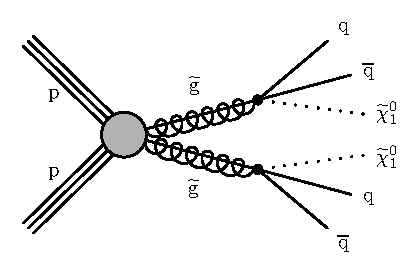
\includegraphics[width=0.3\textwidth]{Supplementary/T1qqqq_feyn_aux}
            \label{fig:T1qqqq_feyn}
        }~~
        \subfigure[T2qq]{
            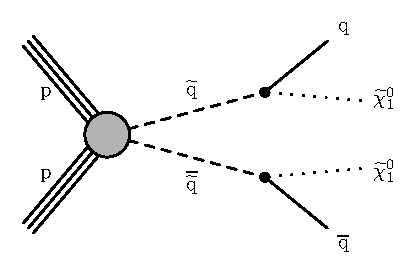
\includegraphics[width=0.3\textwidth]{Supplementary/T2qq_feyn_aux}
            \label{fig:T2qq_feyn}
        }~~
        \caption{
            Graphical representation of the production and decay of
            supersymmetric particles in ``light-flavour models'', i.e. with
            gluinos/squarks decaying to light quarks.
        }
        \label{fig:simplified-models-feyn-light}
    \end{center}
\end{figure}

\begin{figure}[h!]
    \begin{center}
        \subfigure[T1bbbb]{
            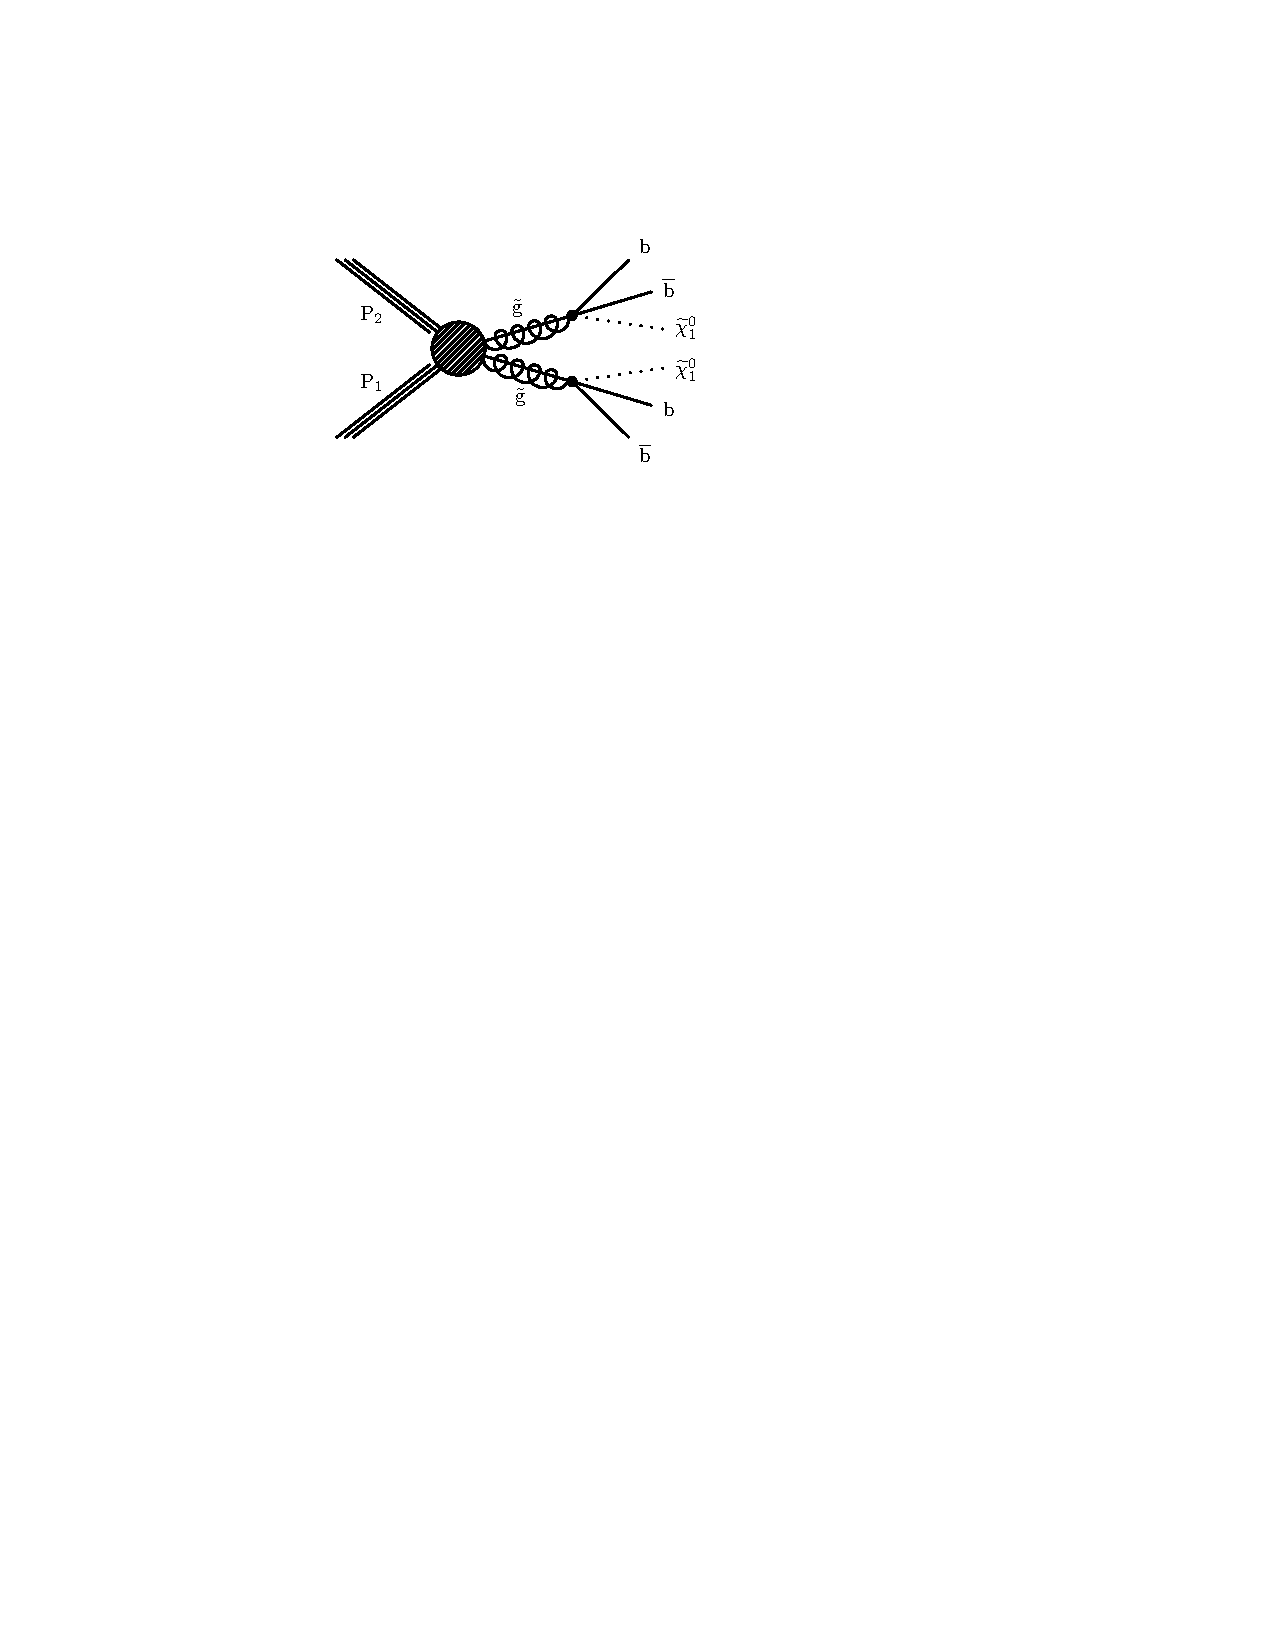
\includegraphics[width=0.3\textwidth]{Supplementary/T1bbbb_feyn_aux}
            \label{fig:T1bbbb_feyn}
        }~~
        \subfigure[T1tttt]{
            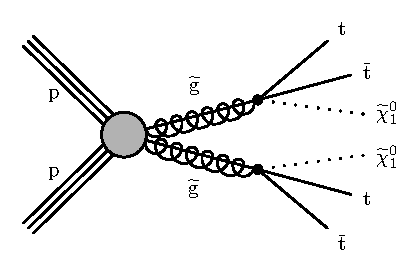
\includegraphics[width=0.3\textwidth]{Supplementary/T1tttt_feyn_aux}
            \label{fig:T1tttt_feyn}
        }~~
        \caption{
            Graphical representation of the production and decay of
            supersymmetric particles in gluino models with decoupled third
            generation squarks.
        }
        \label{fig:simplified-models-feyn-gluino}
    \end{center}
\end{figure}

\begin{figure}[h!]
    \begin{center}
        \subfigure[T2bb]{
            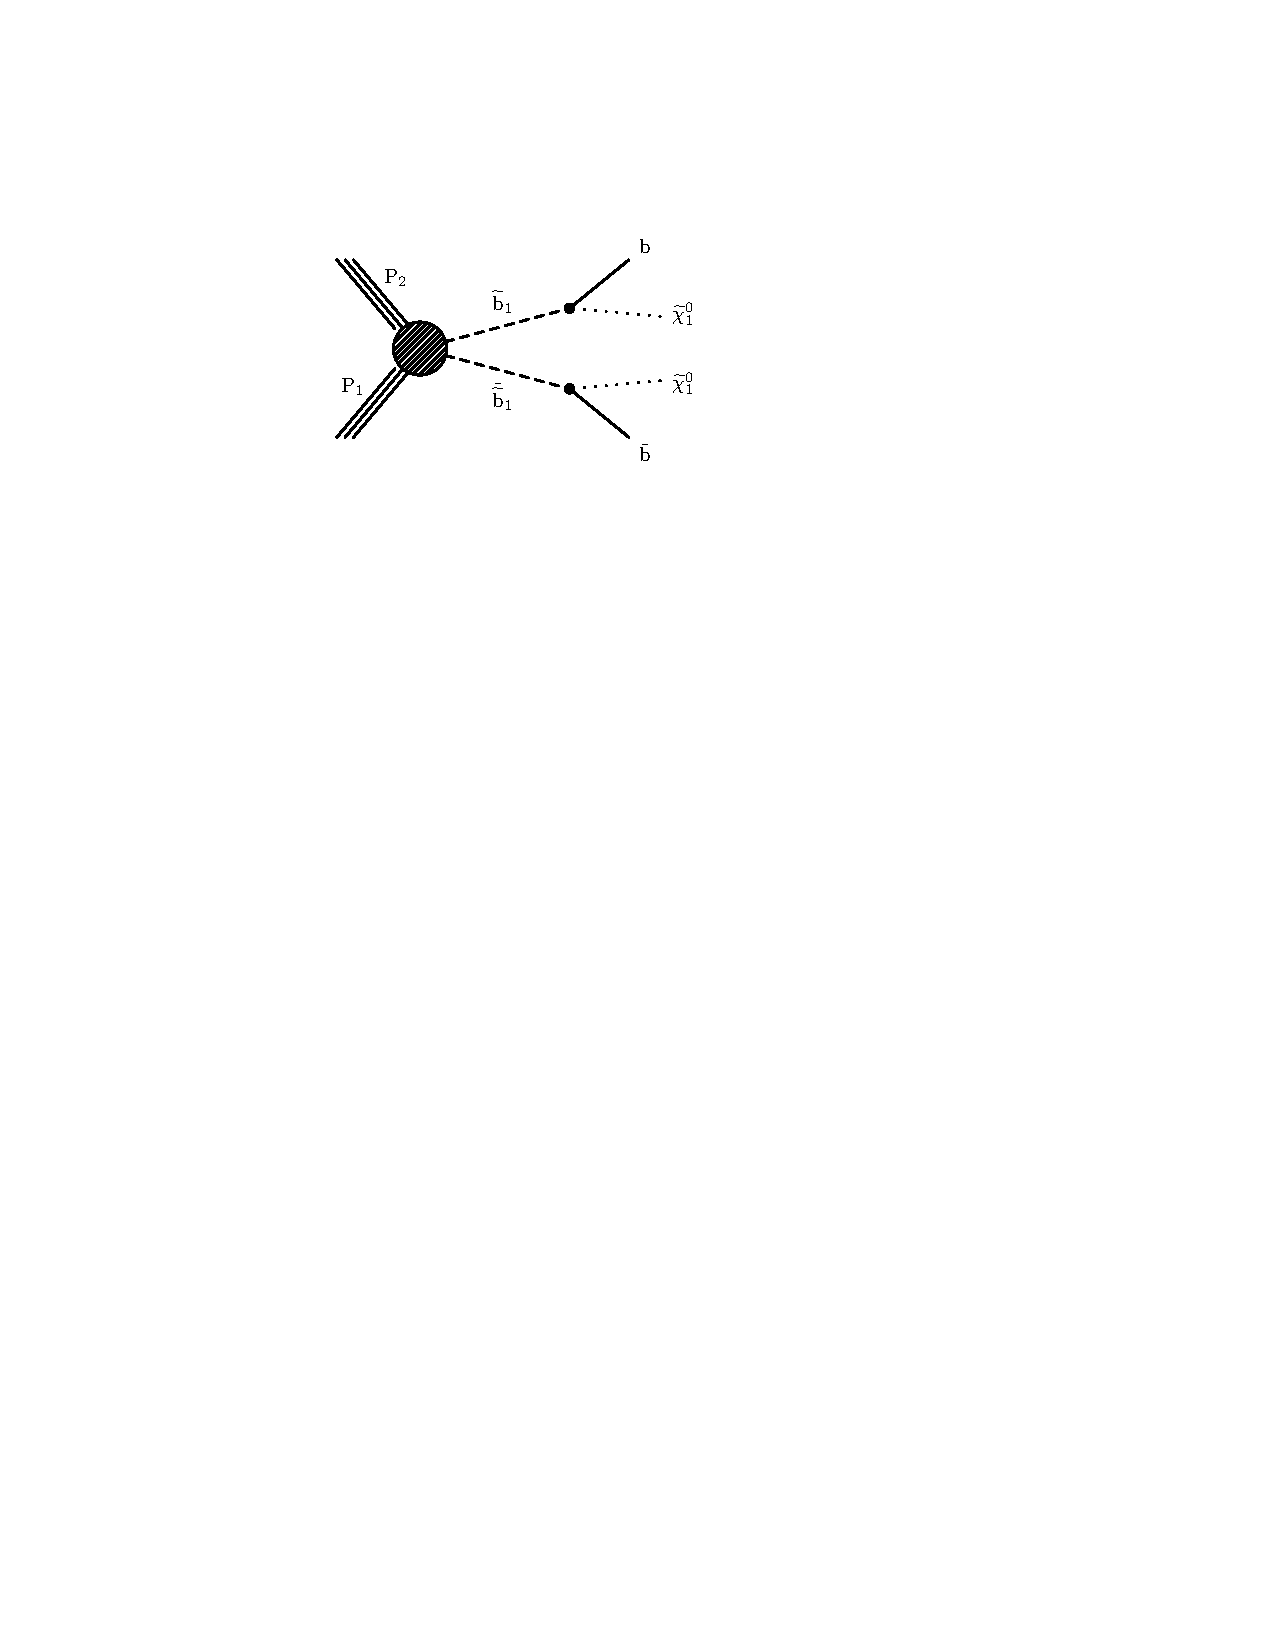
\includegraphics[width=0.3\textwidth]{Supplementary/T2bb_feyn_aux}
            \label{fig:T2bb_feyn}
        }~~
        \subfigure[T2tt]{
            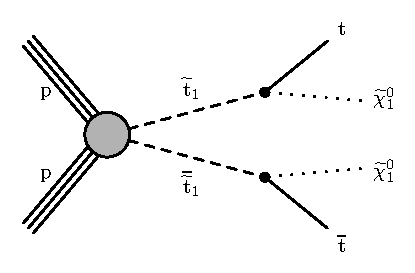
\includegraphics[width=0.3\textwidth]{Supplementary/T2tt_feyn_aux}
            \label{fig:T2tt_feyn}
        }~~
        \subfigure[T2cc]{
            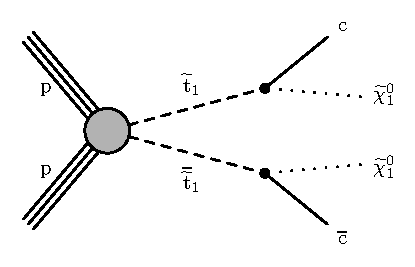
\includegraphics[width=0.3\textwidth]{Supplementary/T2cc_feyn_aux}
            \label{fig:T2cc_feyn}
        }~~
        \caption{
            Graphical representation of the production and decay of
            supersymmetric particles in models with the production of third
            generation squarks (stops and sbottoms).
        }
        \label{fig:simplified-models-feyn-3rdGen}
    \end{center}
\end{figure}

\clearpage
\begin{figure}
  \centering
  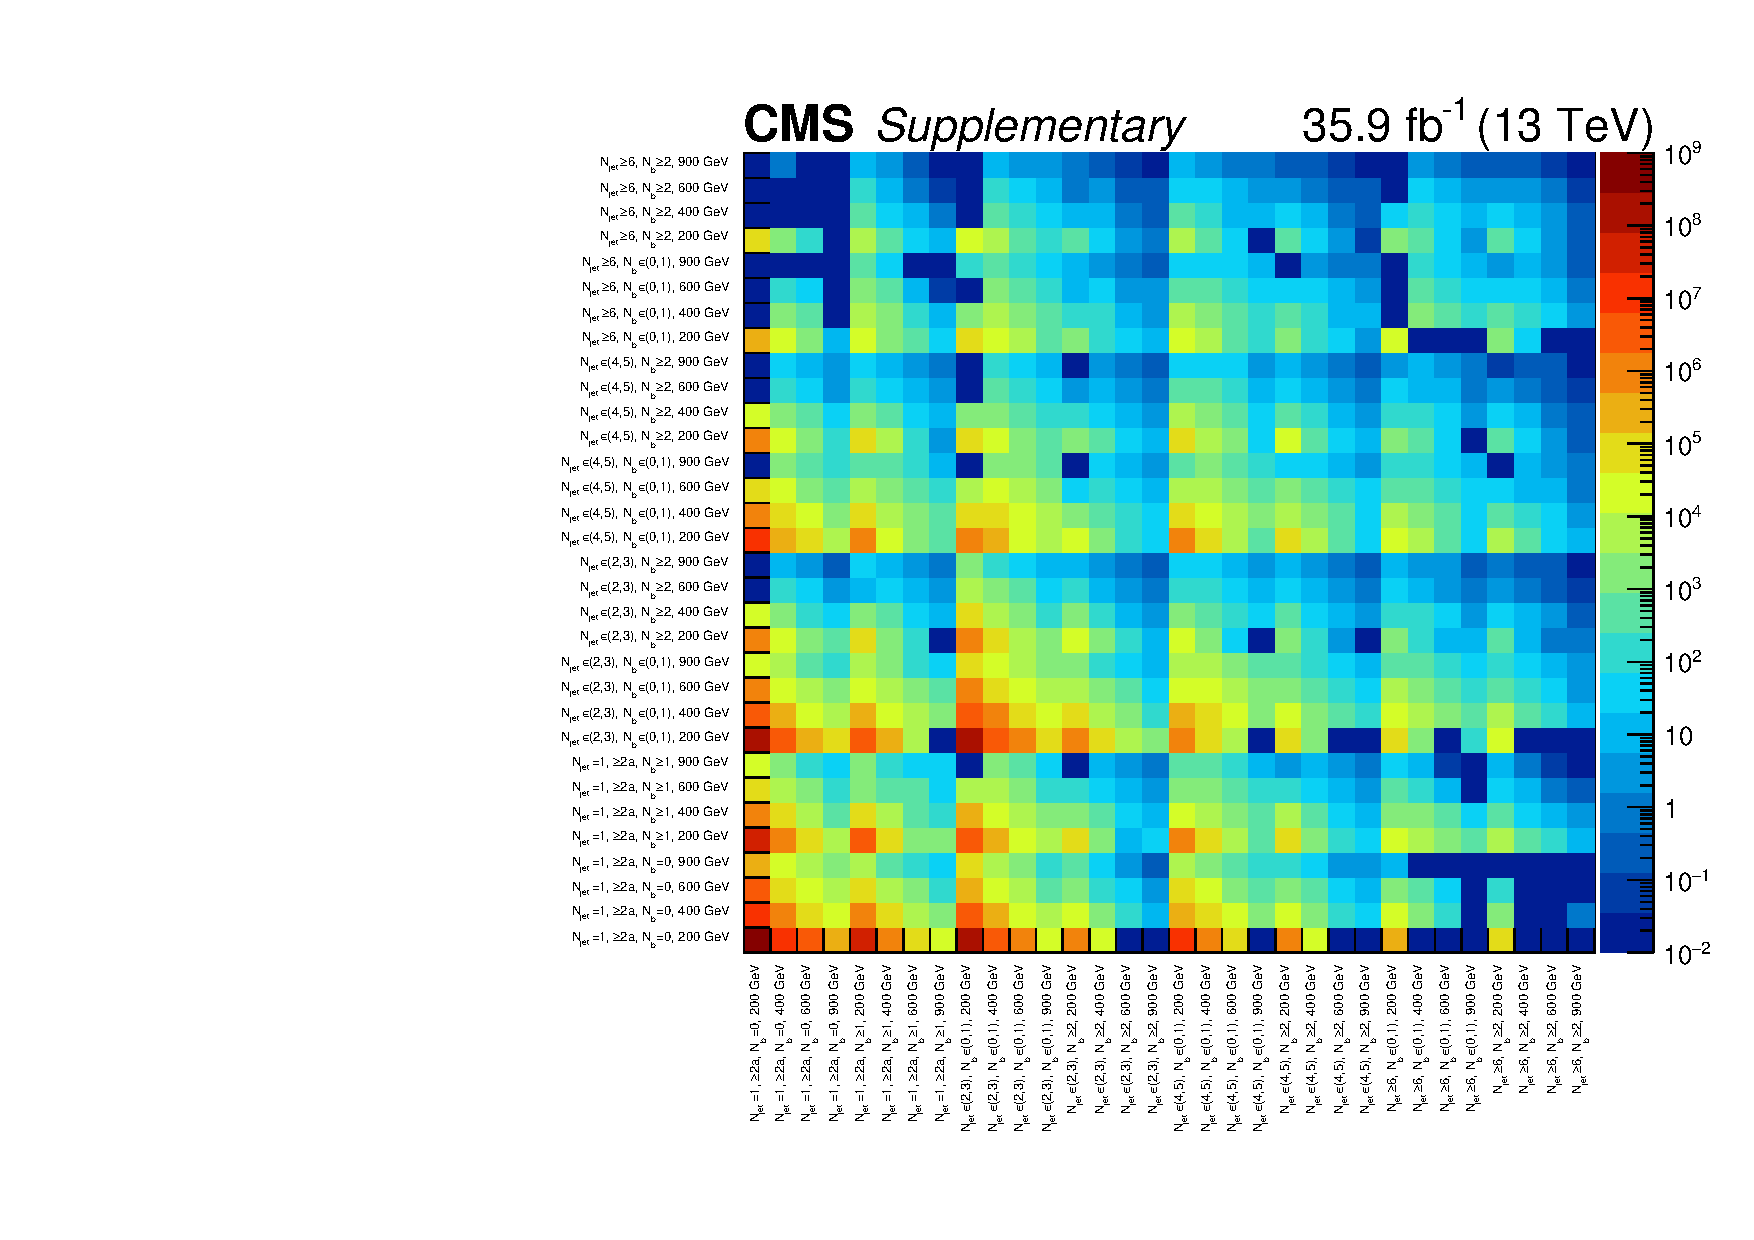
\includegraphics[width=\textwidth]{Supplementary/covariance_aux}
  \caption{Covariance matrix for the SM background estimates obtained
    using the simplified binning schema, determined from the CR-only
    fit.  }
  \label{fig:covariance_aux}
\end{figure} 

\clearpage
\begin{figure}[h!]
  \centering
  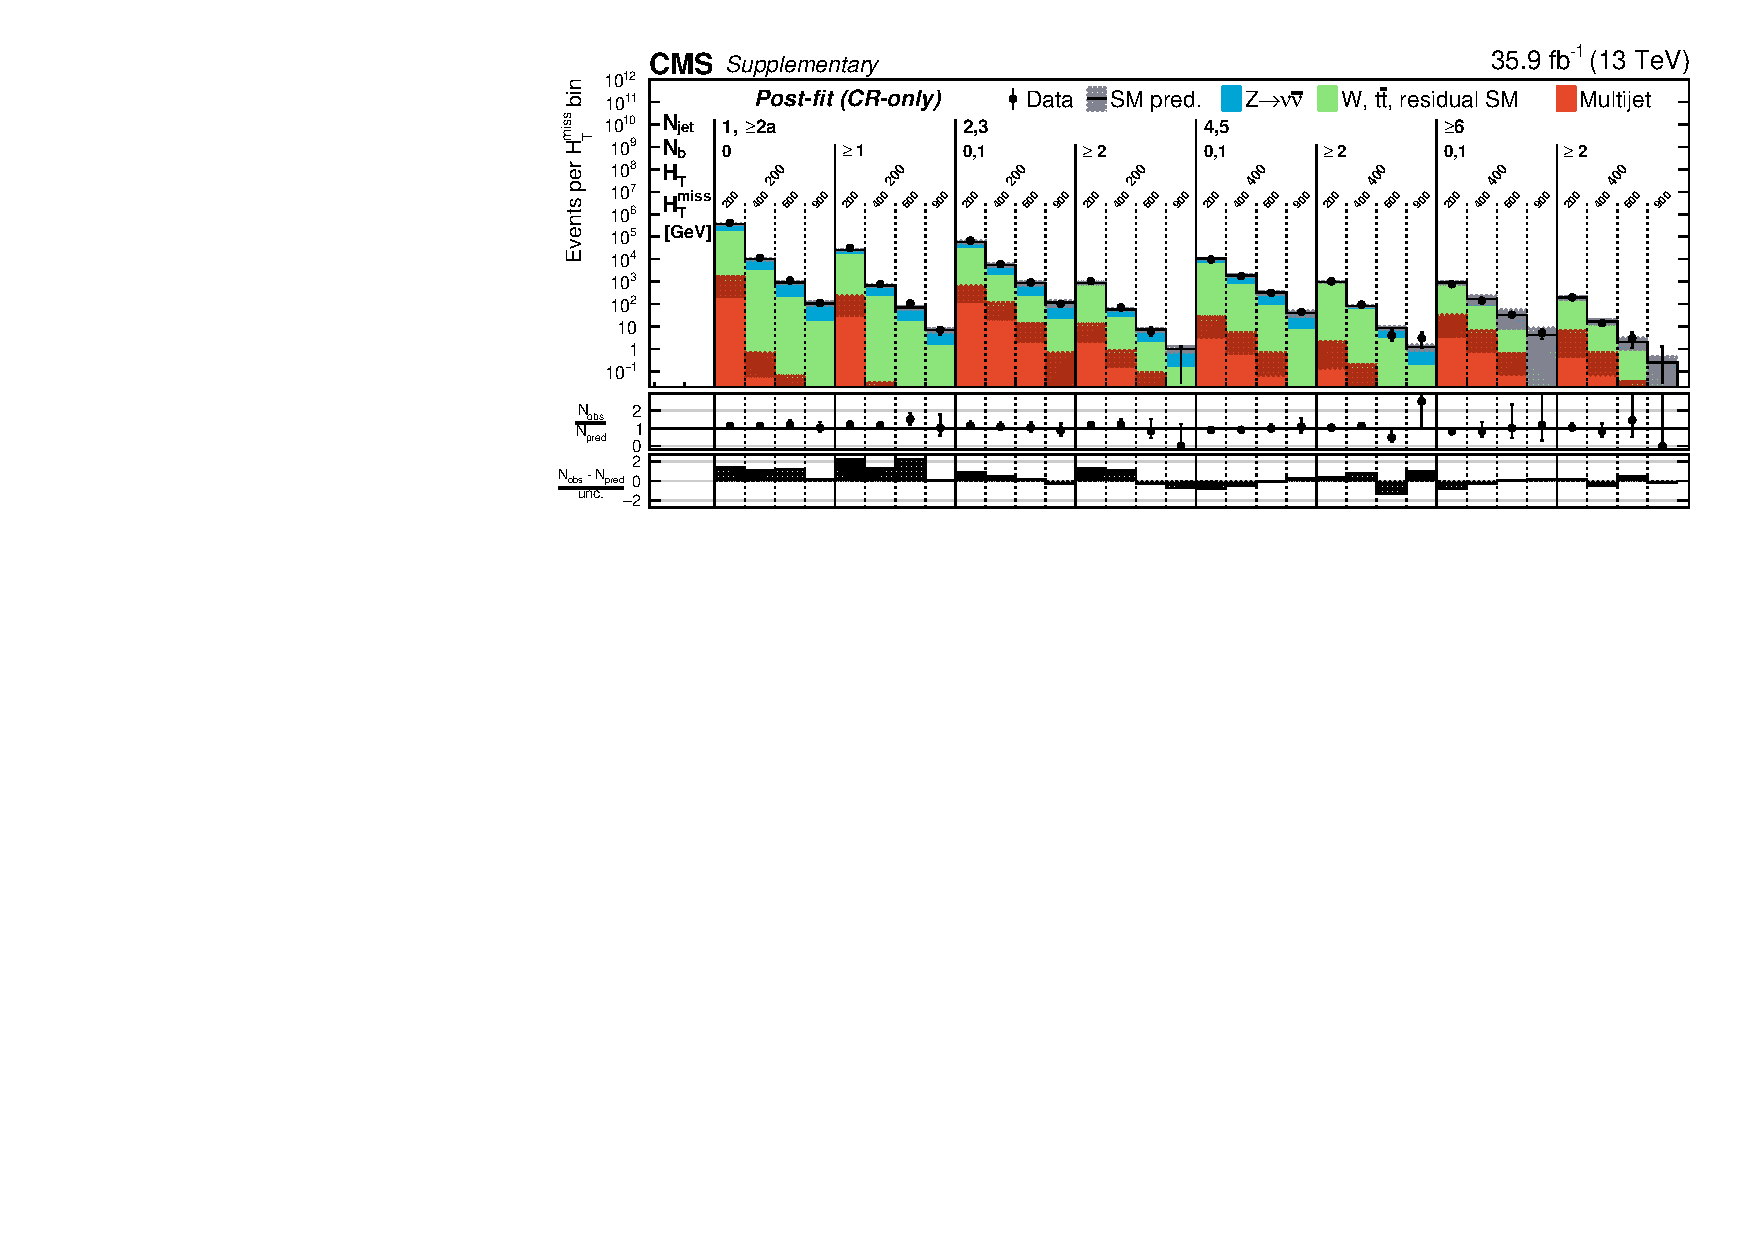
\includegraphics[width=0.95\linewidth]{Supplementary/SimplifiedBinning_results_cr-only-fit_aux} 
  \caption{Results of the CR-only fit based on the simplified binning
    schema. (Top panel) Event yields in data and SM
    expectations. (Centre panel) Ratio of the observed and expected
    counts. (Bottom panel) Observed pulls of the data from
    expectation. Detailed descriptions are given in the text.
  }
  \label{fig:aggregated_results}
\end{figure}

\clearpage
\begin{table}
	\topcaption{Expected and observed limits on the production cross section for the benchmark simplified models using the simplified binning scheme}
  \label{tab:benchmarks_aux}
  \centering
    \begin{tabular}{ lrrcc }
      \hline
      Family
      & $(m_{\text{SUSY}}, m_{\mathrm{LSP}})$
      & \multicolumn{2}{c}{$\mu$ (95\% CL)}                                                                            \\ [0.3ex]
      ($c\tau$)
      & [\GeVns{}]
      & Exp.
      & Obs.                                                                                                           \\ [0.3ex]
      \hline
      \multirow{2}{*}{\texttt{T1bbbb}}
& (1900, 100) 
& 1.16 & 1.15 \\
& (1300, 1100)
& 0.78 & 1.03 \\ [0.5ex]
      \multirow{2}{*}{\texttt{T1tttt}}
& (1700, 100) 
& 0.67 & 0.70 \\
& (950, 600)  
& 3.39 & 2.95 \\ [0.5ex]
      \multirow{2}{*}{\texttt{T2bb}}
& (800, 50)
%& (1000, 100) % These are the values in the AN
& 0.89 & 0.56 \\
& (375, 300)
%& (550, 450)  % These are the values in the AN
& 1.46 & 1.05 \\ [0.5ex]
      \multirow{3}{*}{\texttt{T2tt}}
& (1000, 50)  
& 0.96 & 0.88 \\
& (450, 200)  
& 1.25 & 1.07 \\ 
& (250, 150)  
& 3.14 & 2.86 \\ [0.5ex]
      \multirow{1}{*}{\texttt{T2cc}}
& (500, 480)  
& 1.52 & 2.43 \\ [0.5ex]
      \multirow{2}{*}{\texttt{T2qq\_8fold}}
& (1250, 100) 
& 0.91 & 0.72 \\
& (700, 600)  
& 1.81 & 2.48 \\ [0.5ex]
      \multirow{2}{*}{\texttt{T2qq\_1fold}}
& (700, 100)  
& 1.07 & 2.20 \\
& (400, 300)  
& 1.60 & 1.60 \\ [0.5ex]
      \texttt{T1qqqqLL}
& (1800, 200)
& 1.36 & 2.00 \\
     ($10^{-3}\unit{mm}$)
& (1000, 900)
& 1.46 & 2.40 \\ [0.5ex]
      \texttt{T1qqqqLL}
& (1800, 200)
& 0.52 & 0.60 \\
     ($1\unit{mm}$)
& (1000, 900)
& 0.41 & 0.47 \\ [0.5ex]
      \texttt{T1qqqqLL}
& (1000, 200)
& 1.23 & 1.40 \\
     ($100\,000\unit{mm}$)
& (1000, 900)
& 1.22 & 1.90 \\
      \hline
    \end{tabular}
\end{table}

\clearpage
\begin{figure}
    \begin{center}
        \subfigure[T1qqqq: the 95\% C.L. observed upper limit on the cross section
            (histogram), with the expected (solid black line) observed
            (solid red line) exclusion contours.]{
            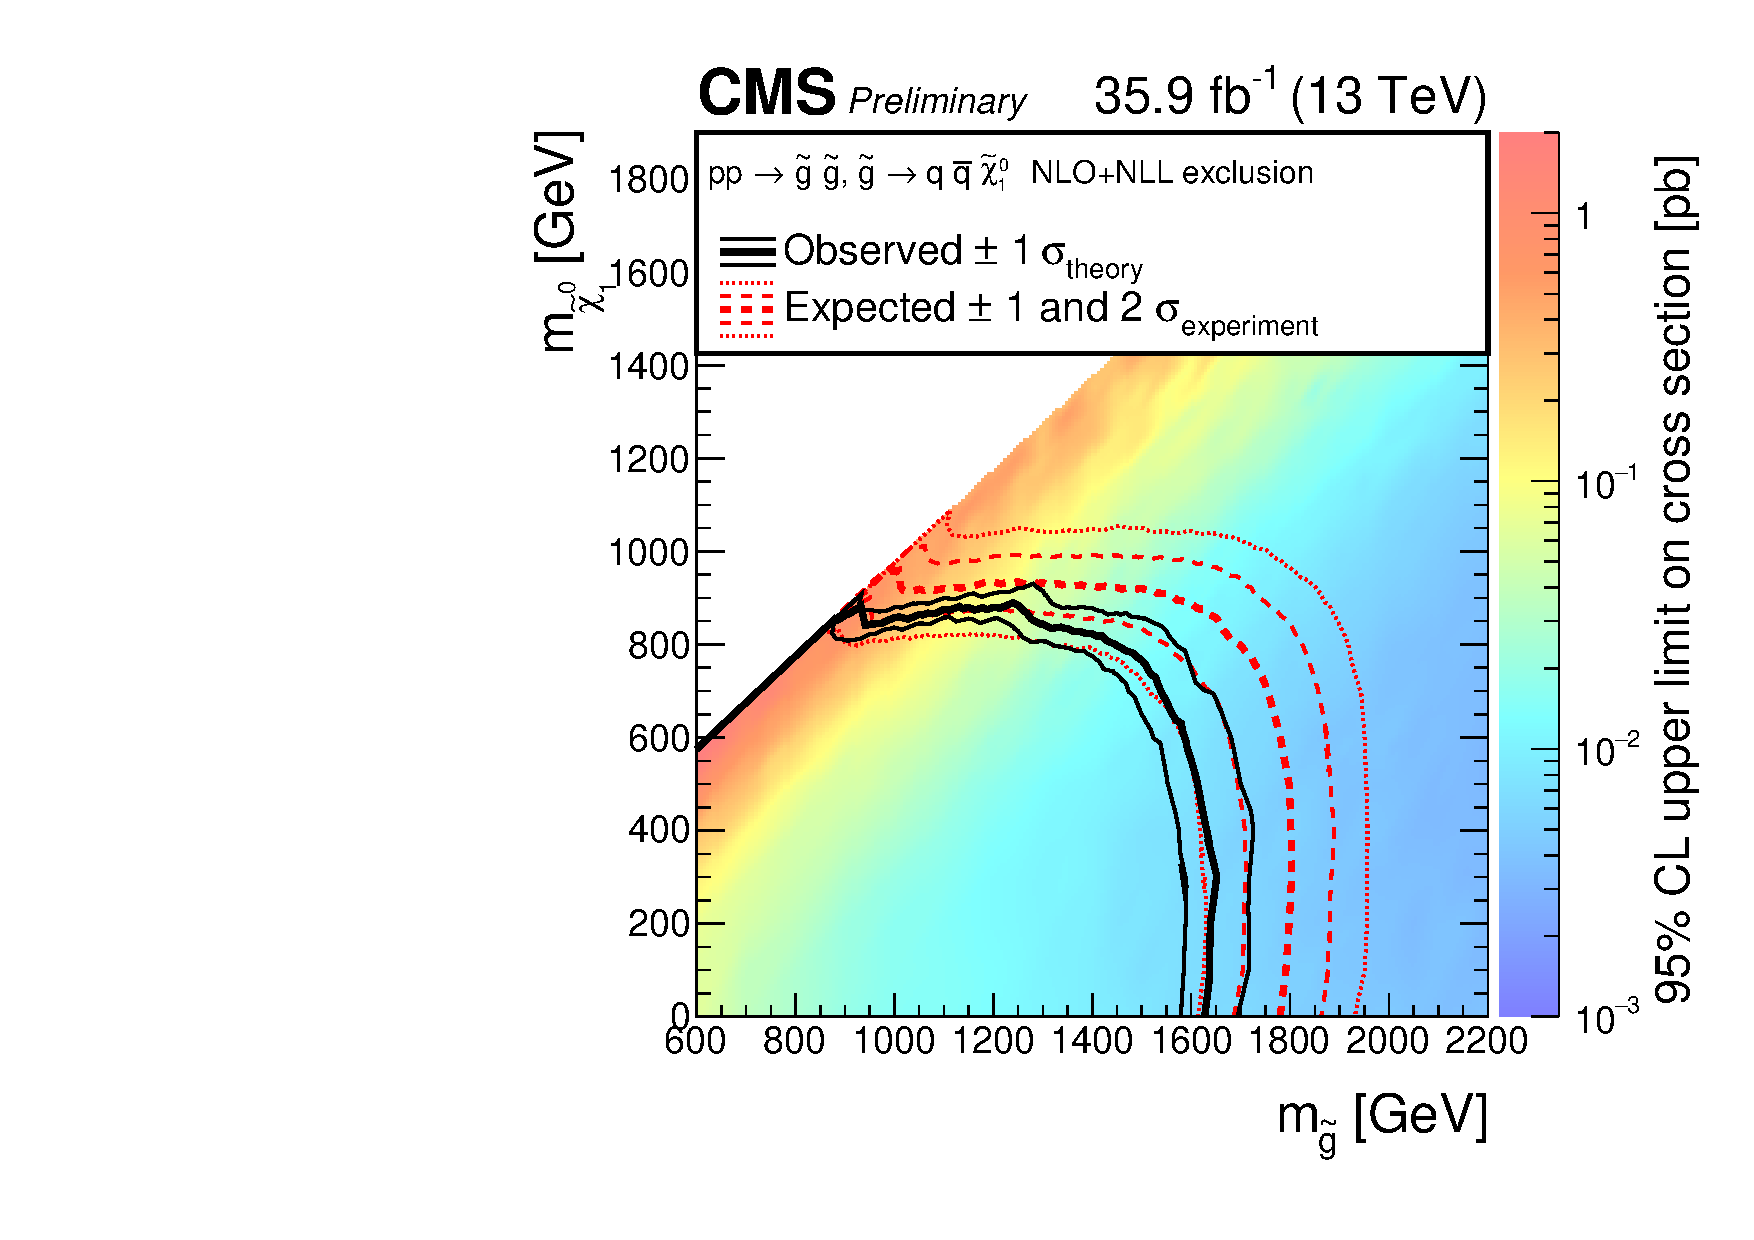
\includegraphics[width=0.4\textwidth]{Supplementary/T1qqqqXSEC}
            \label{fig:T1qqqq_excl}
        } ~~
        \subfigure[T1qqqq: signal acceptance
            including all jet categories.]{
            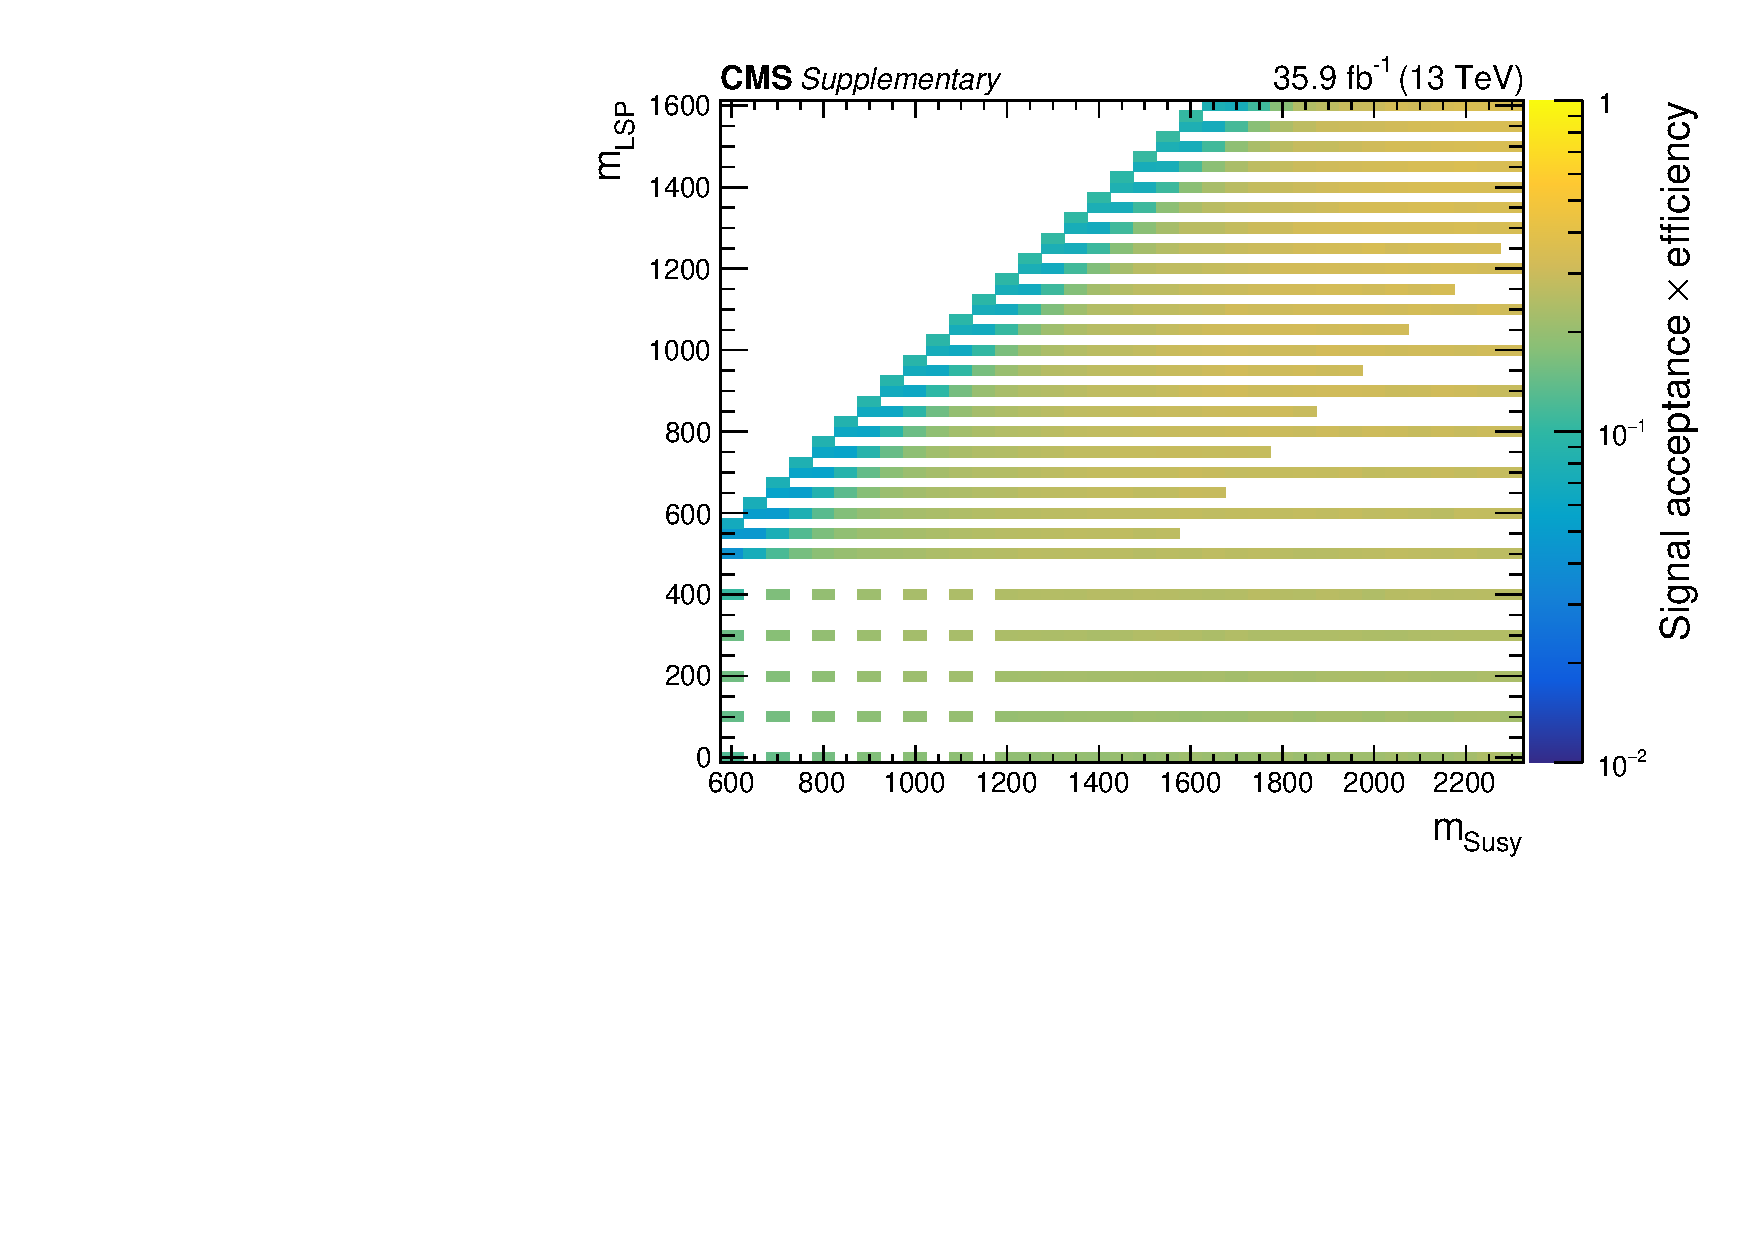
\includegraphics[width=0.52\textwidth]{Supplementary/T1qqqqEFF_aux}
            \label{fig:T1qqqq_eff}
        }
        \caption{The 95\% C.L. observed upper limit on the cross section
            (heat-map), with the expected (solid black line) observed
            (solid red line) exclusion contours, and the signal acceptance
            including all jet categories for the T1qqqq model.
        }
        \label{fig:T1qqqq}
    \end{center}
\end{figure}

\begin{figure}
    \begin{center}
        \subfigure[T1bbbb: the 95\% C.L. observed upper limit on the cross section
            (histogram), with the expected (solid black line) observed
            (solid red line) exclusion contours.]{
            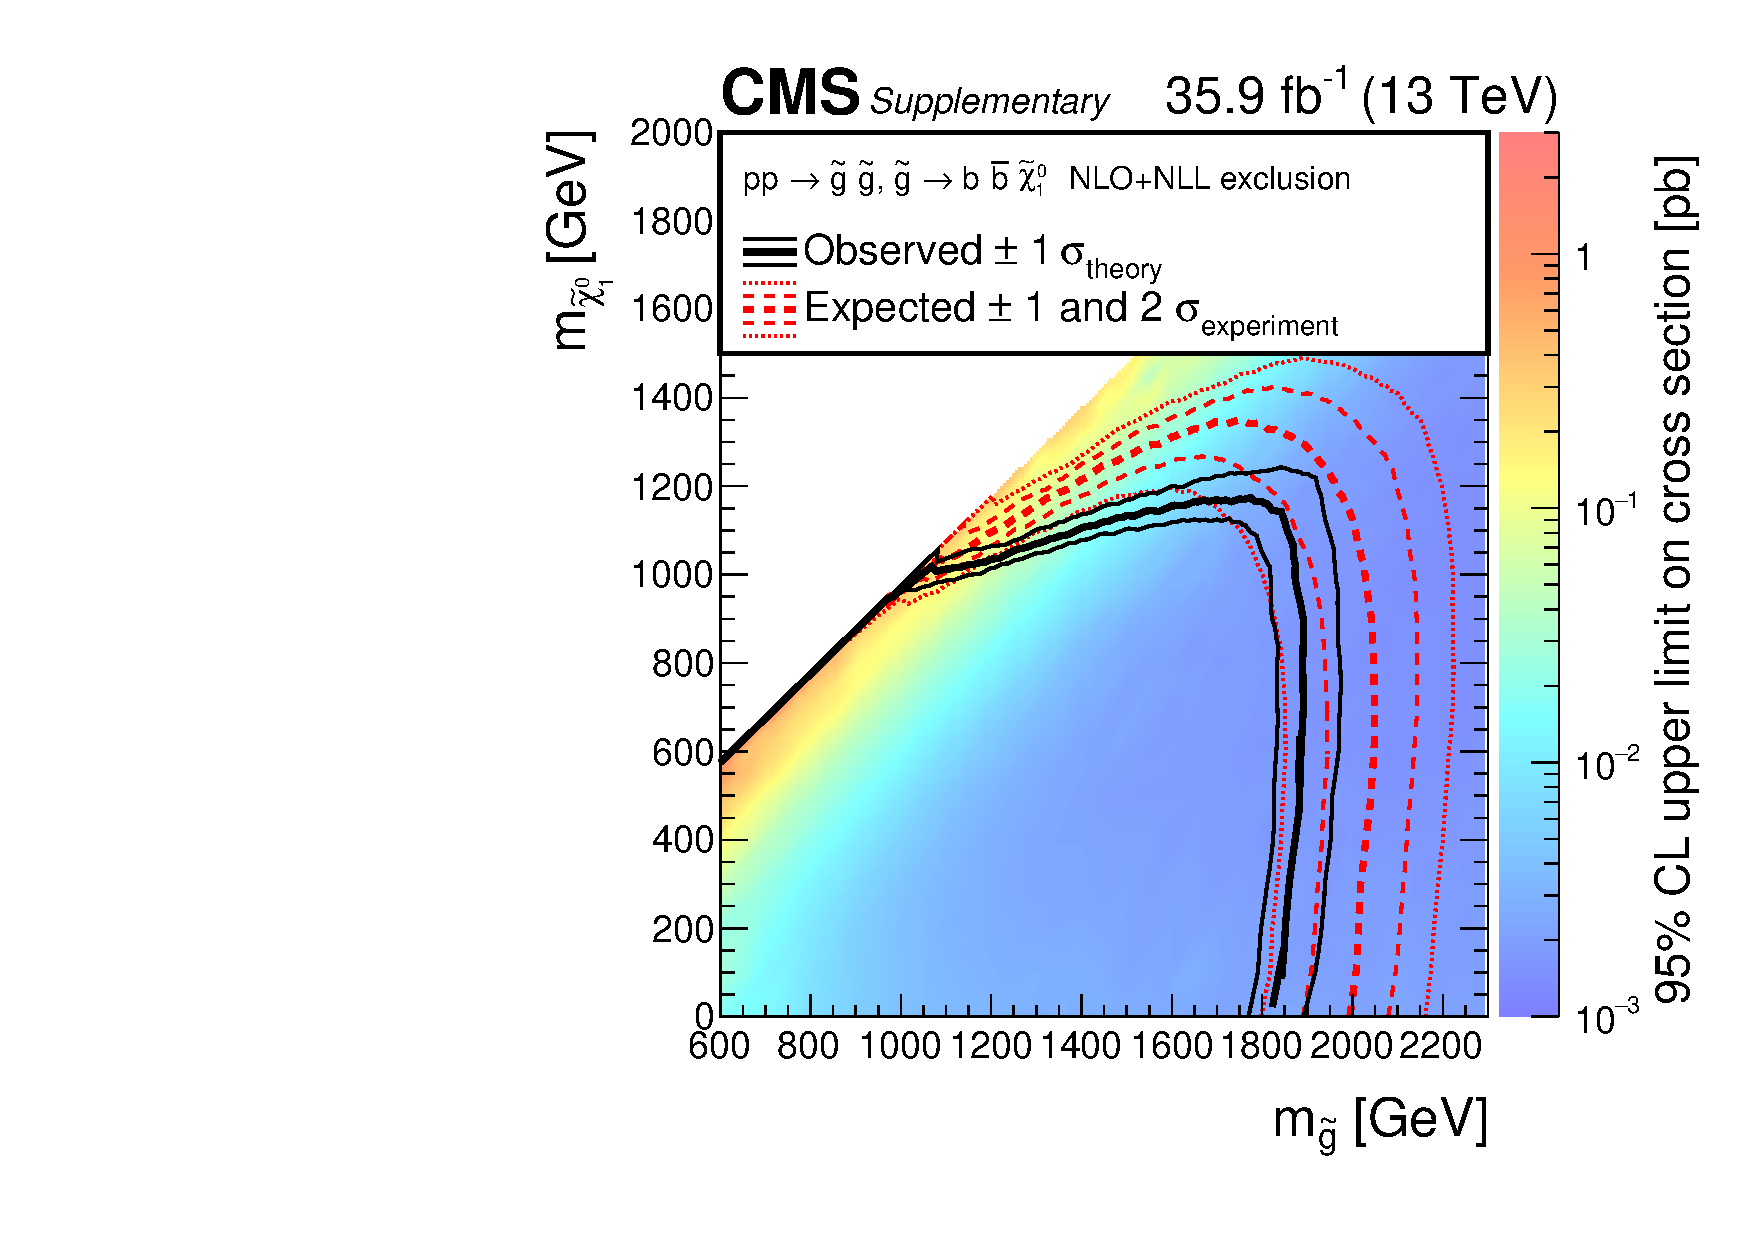
\includegraphics[width=0.4\textwidth]{Supplementary/T1bbbbXSEC}
            \label{fig:T1bbbb_excl}
        } ~~
        \subfigure[T1bbbb: signal acceptance
            including all jet categories.]{
            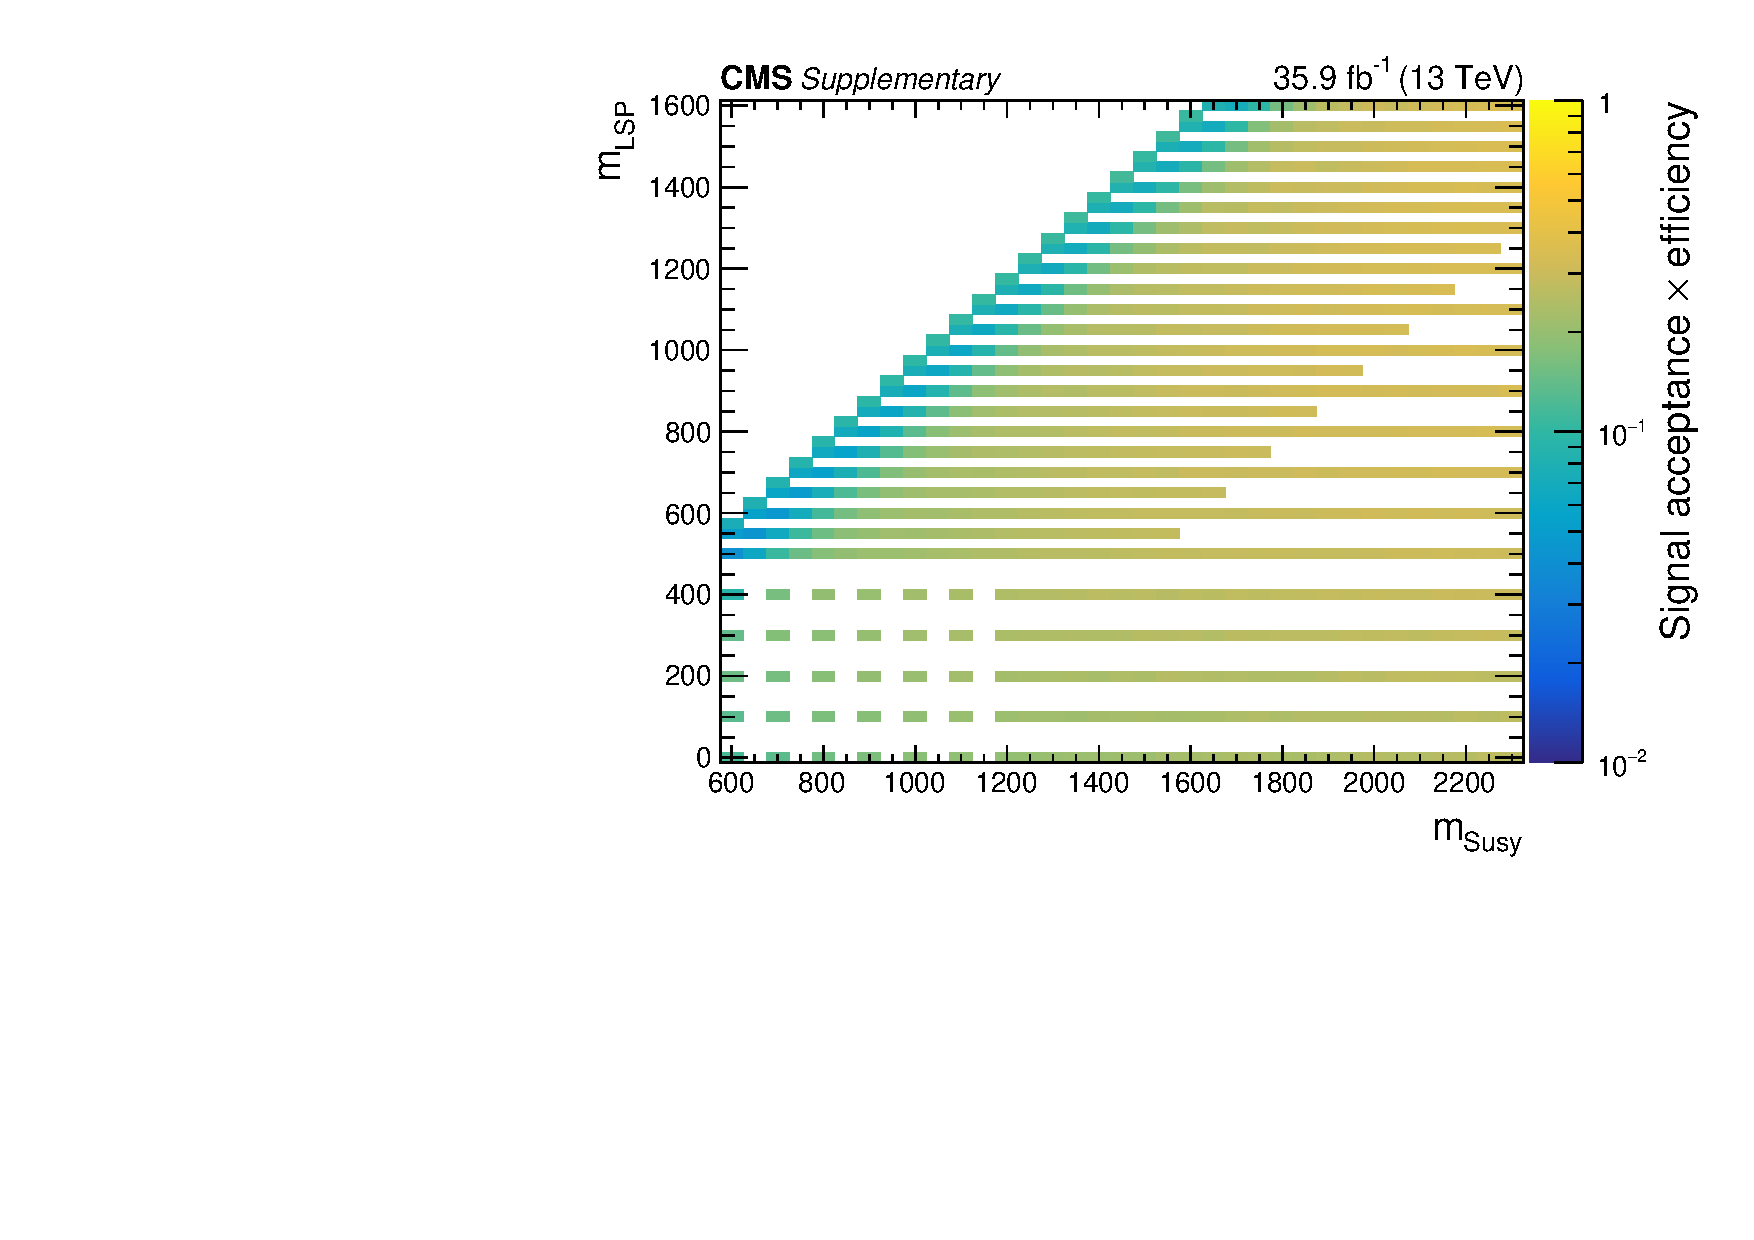
\includegraphics[width=0.52\textwidth]{Supplementary/T1bbbbEFF_aux}
            \label{fig:T1bbbb_eff}
        }
        \caption{The 95\% C.L. observed upper limit on the cross section
            (heat-map), with the expected (solid black line) observed
            (solid red line) exclusion contours, and the signal acceptance
            including all jet categories for the T1bbbb model.
        }
        \label{fig:T1bbbb}
    \end{center}
\end{figure}

\begin{figure}
    \begin{center}
        \subfigure[T1tttt: the 95\% C.L. observed upper limit on the cross section
            (histogram), with the expected (solid black line) observed
            (solid red line) exclusion contours.]{
            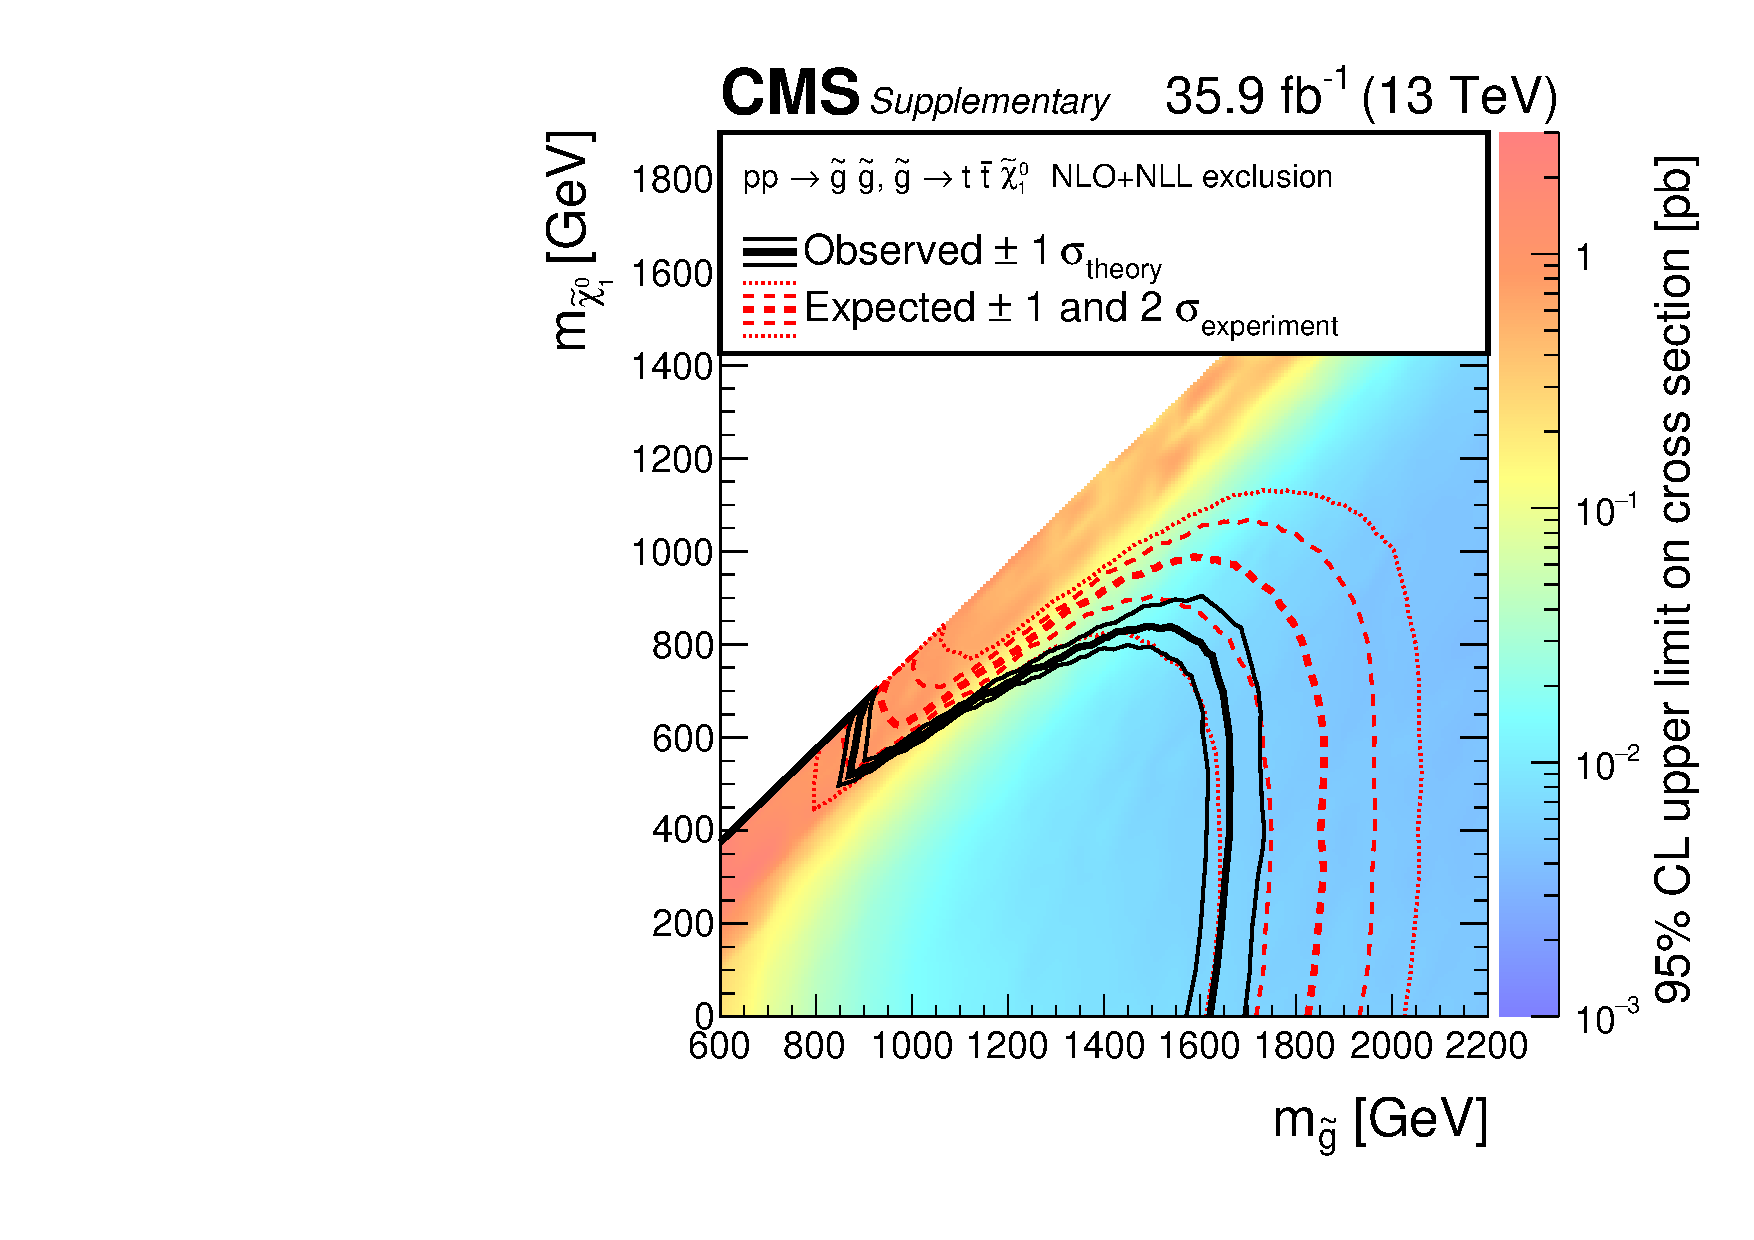
\includegraphics[width=0.4\textwidth]{Supplementary/T1ttttXSEC}
            \label{fig:T1tttt_excl}
        } ~~
        \subfigure[T1tttt: signal acceptance
            including all jet categories.]{
            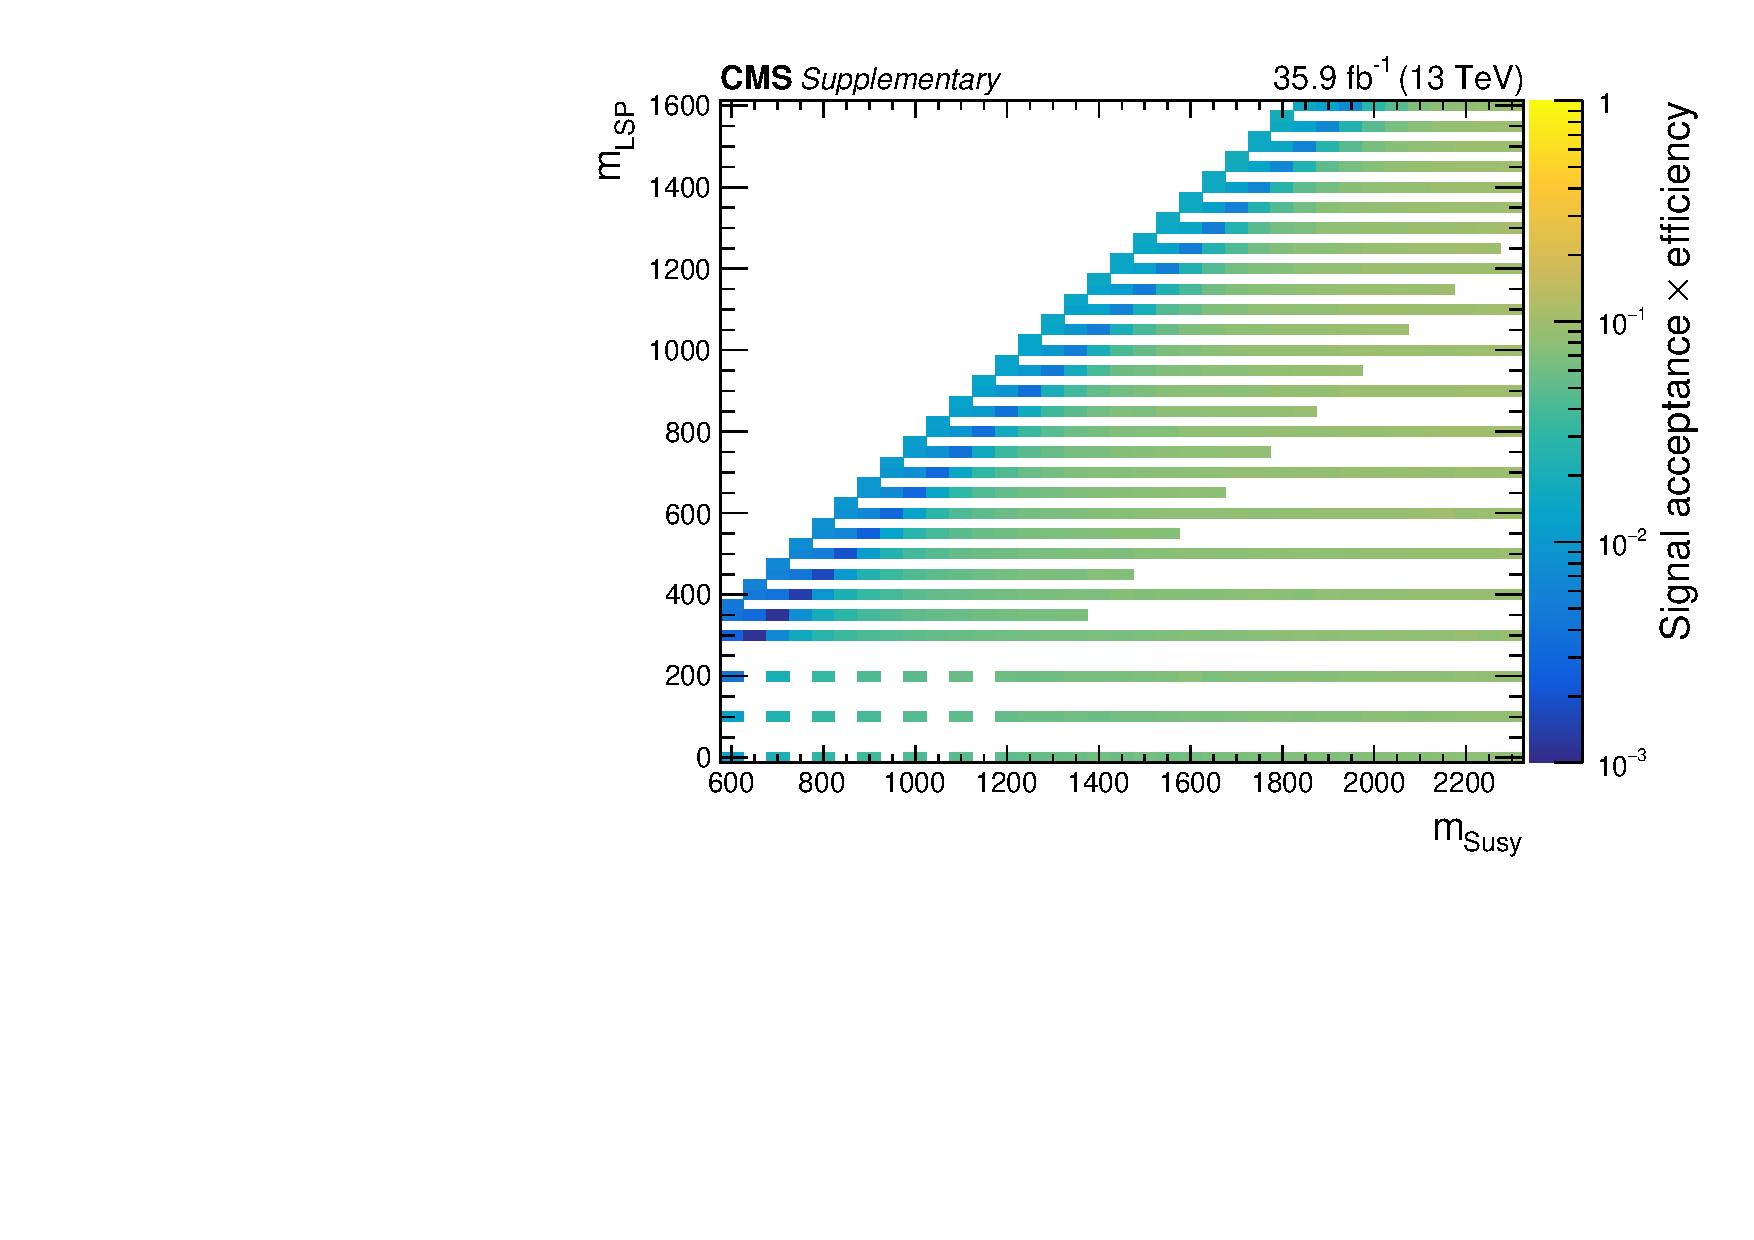
\includegraphics[width=0.52\textwidth]{Supplementary/T1ttttEFF_aux}
            \label{fig:T1tttt_eff}
        }
        \caption{The 95\% C.L. observed upper limit on the cross section
            (heat-map), with the expected (solid black line) observed
            (solid red line) exclusion contours, and the signal acceptance
            including all jet categories for the T1tttt model.
        }
        \label{fig:T1tttt}
    \end{center}
\end{figure}

\begin{figure}
    \begin{center}
        \subfigure[T2bb: the 95\% C.L. observed upper limit on the cross section
            (histogram), with the expected (solid black line) observed
            (solid red line) exclusion contours.]{
            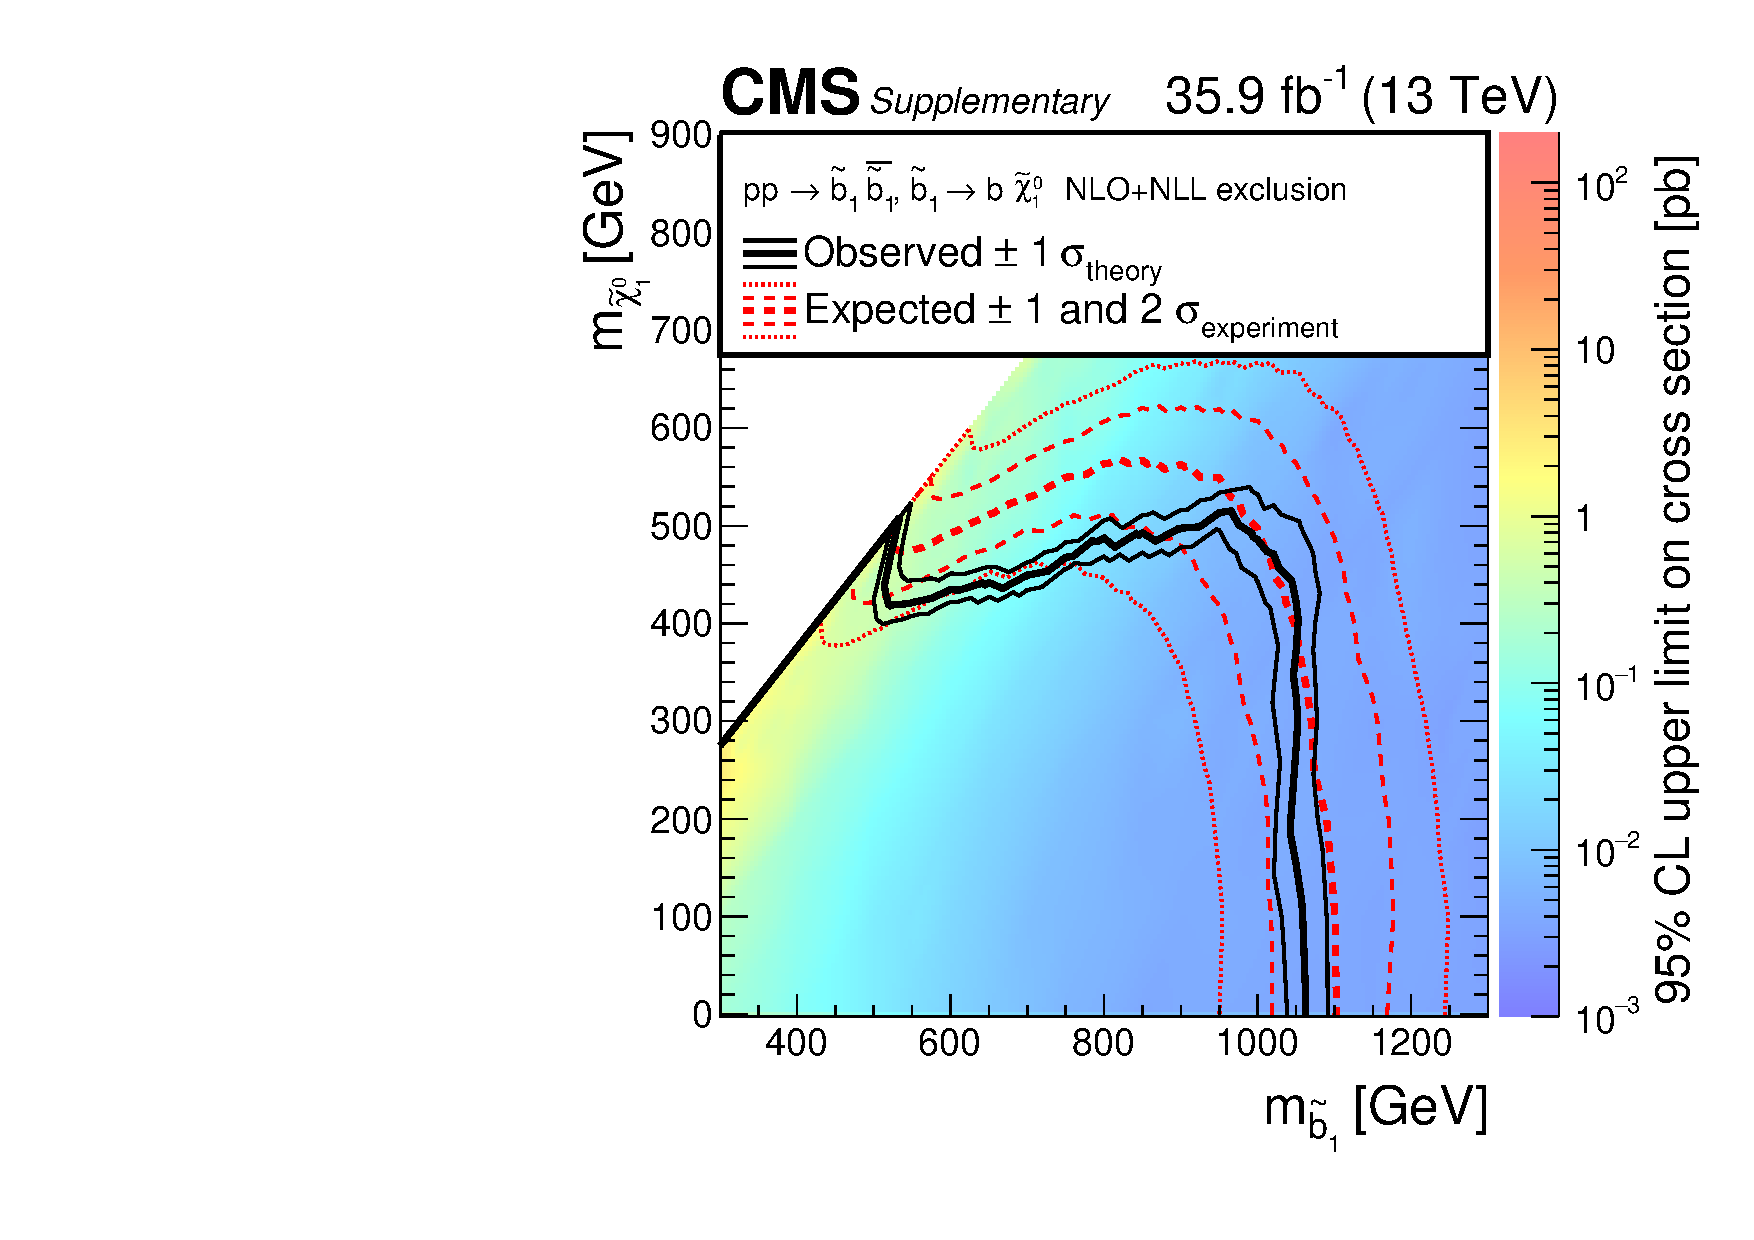
\includegraphics[width=0.4\textwidth]{Supplementary/T2bbXSEC}
            \label{fig:T2bb_excl}
        } ~~
        \subfigure[T2bb: signal acceptance
            including all jet categories.]{
            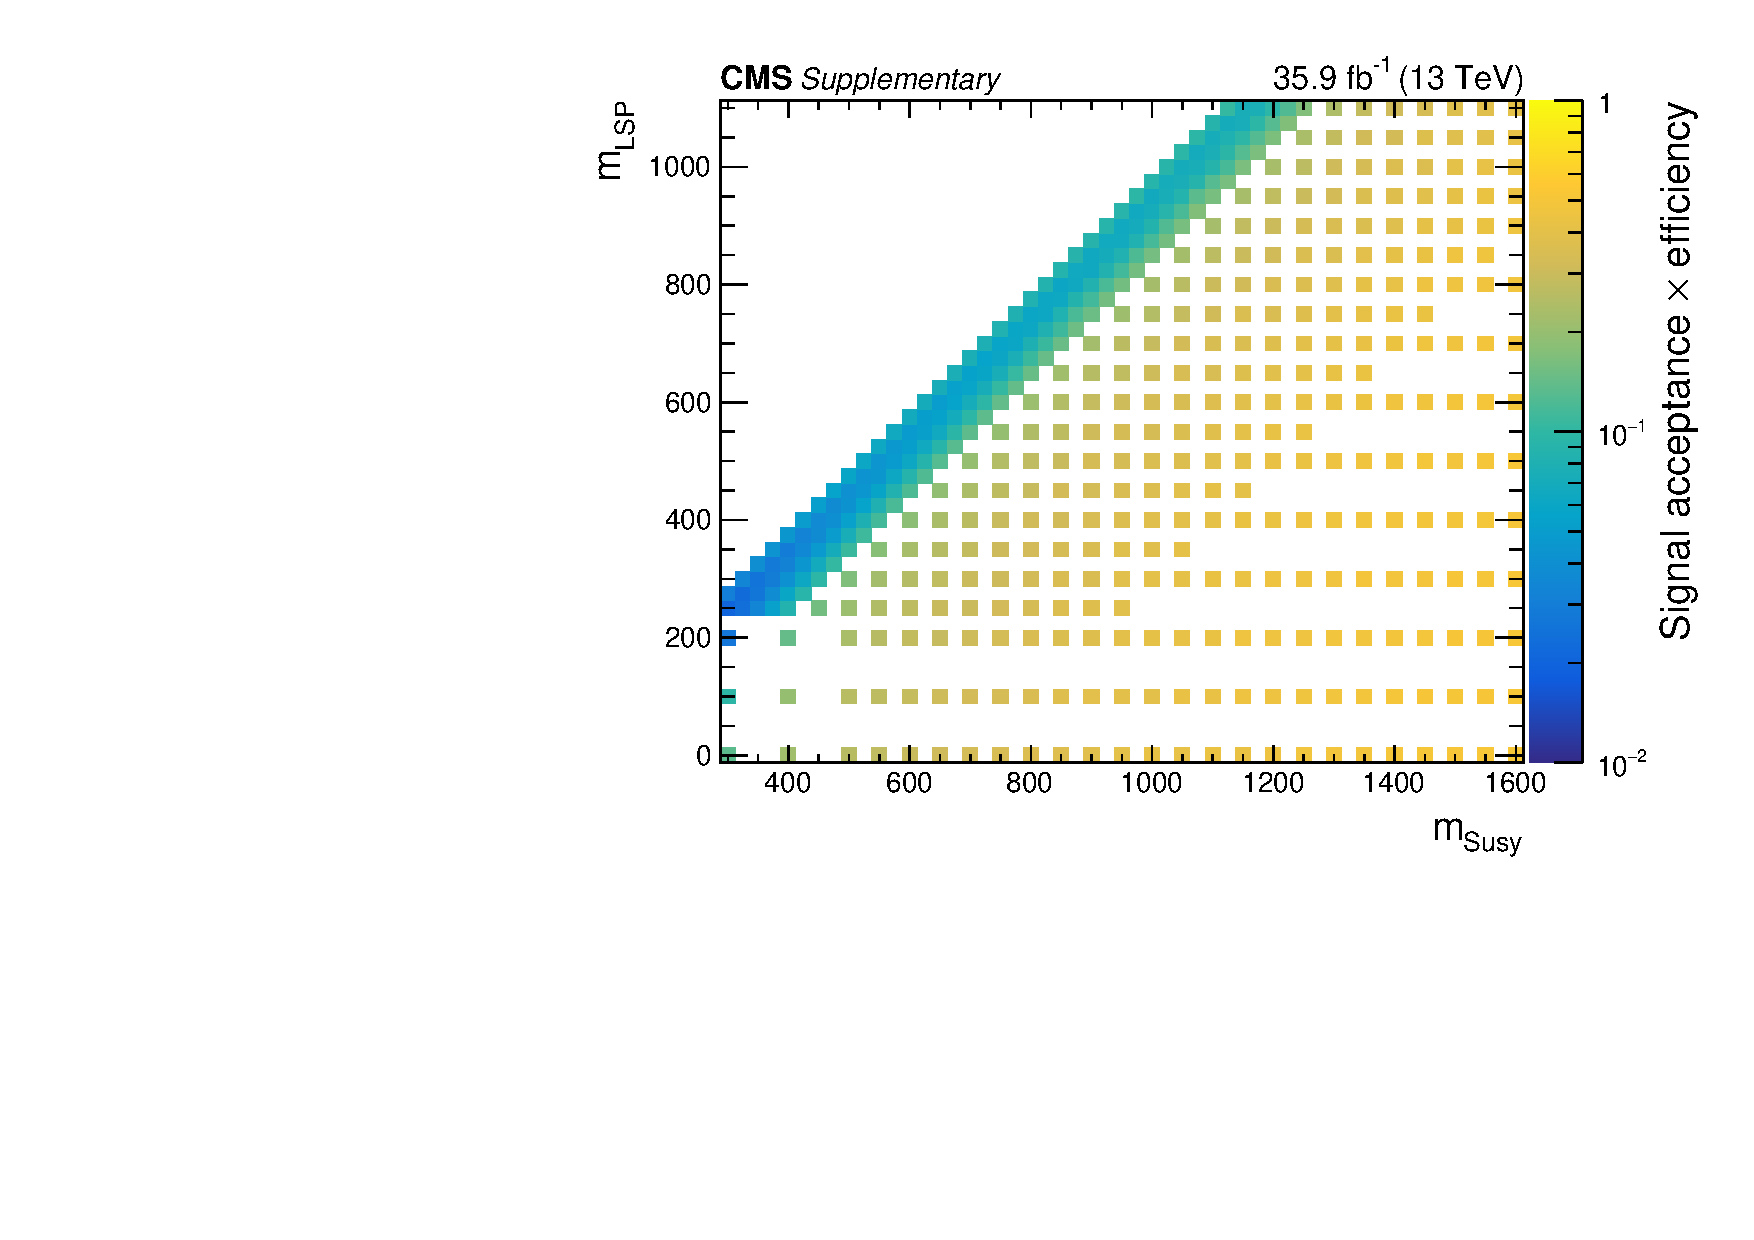
\includegraphics[width=0.52\textwidth]{Supplementary/T2bbEFF_aux}
            \label{fig:T2bb_eff}
        }
        \caption{The 95\% C.L. observed upper limit on the cross section
            (heat-map), with the expected (solid black line) observed
            (solid red line) exclusion contours, and the signal acceptance
            including all jet categories for the T2bb model.
        }
        \label{fig:T2bb}
    \end{center}
\end{figure}

\begin{figure}
    \begin{center}
        \subfigure[T2tt: the 95\% C.L. observed upper limit on the cross section
            (histogram), with the expected (solid black line) observed
            (solid red line) exclusion contours.]{
            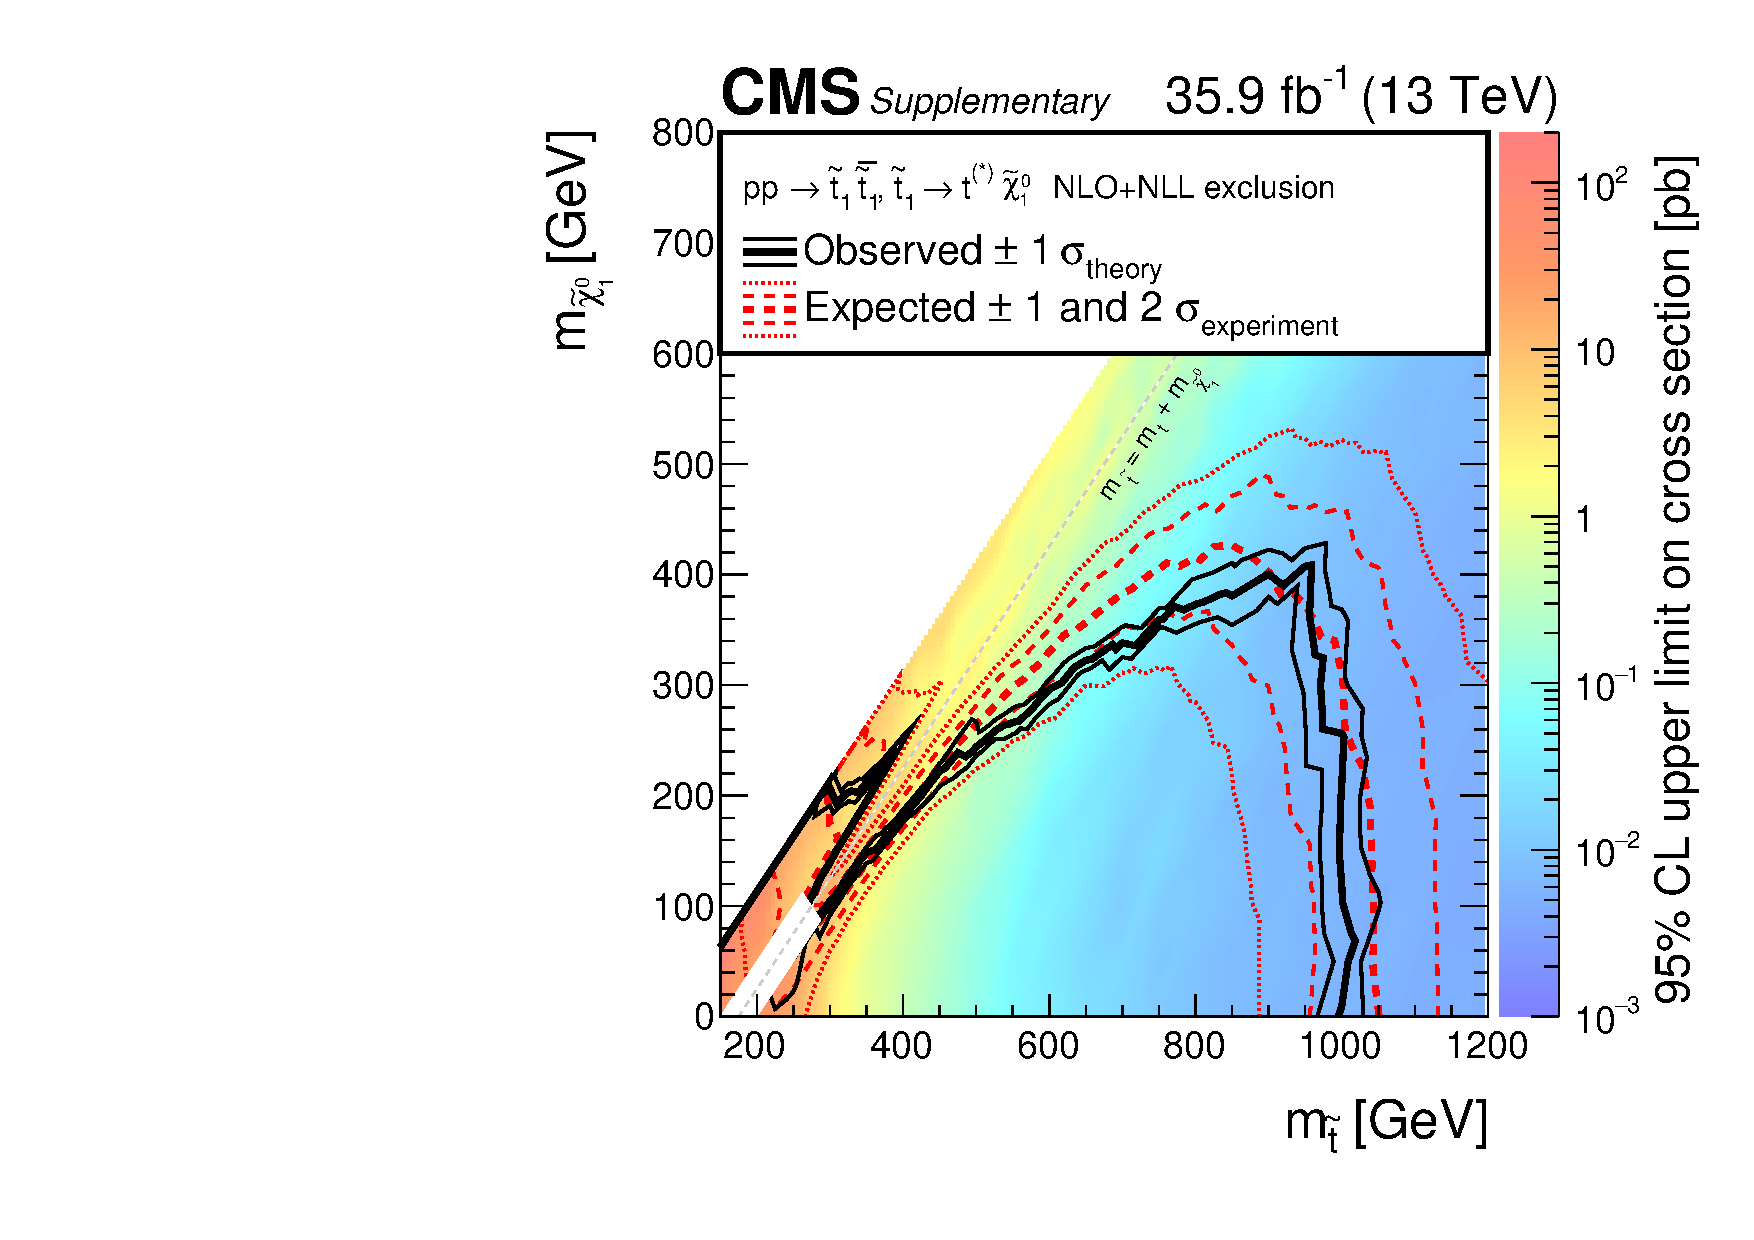
\includegraphics[width=0.4\textwidth]{Supplementary/T2ttXSEC}
            \label{fig:T2tt_excl}
        } ~~
        \subfigure[T2tt: signal acceptance
            including all jet categories.]{
            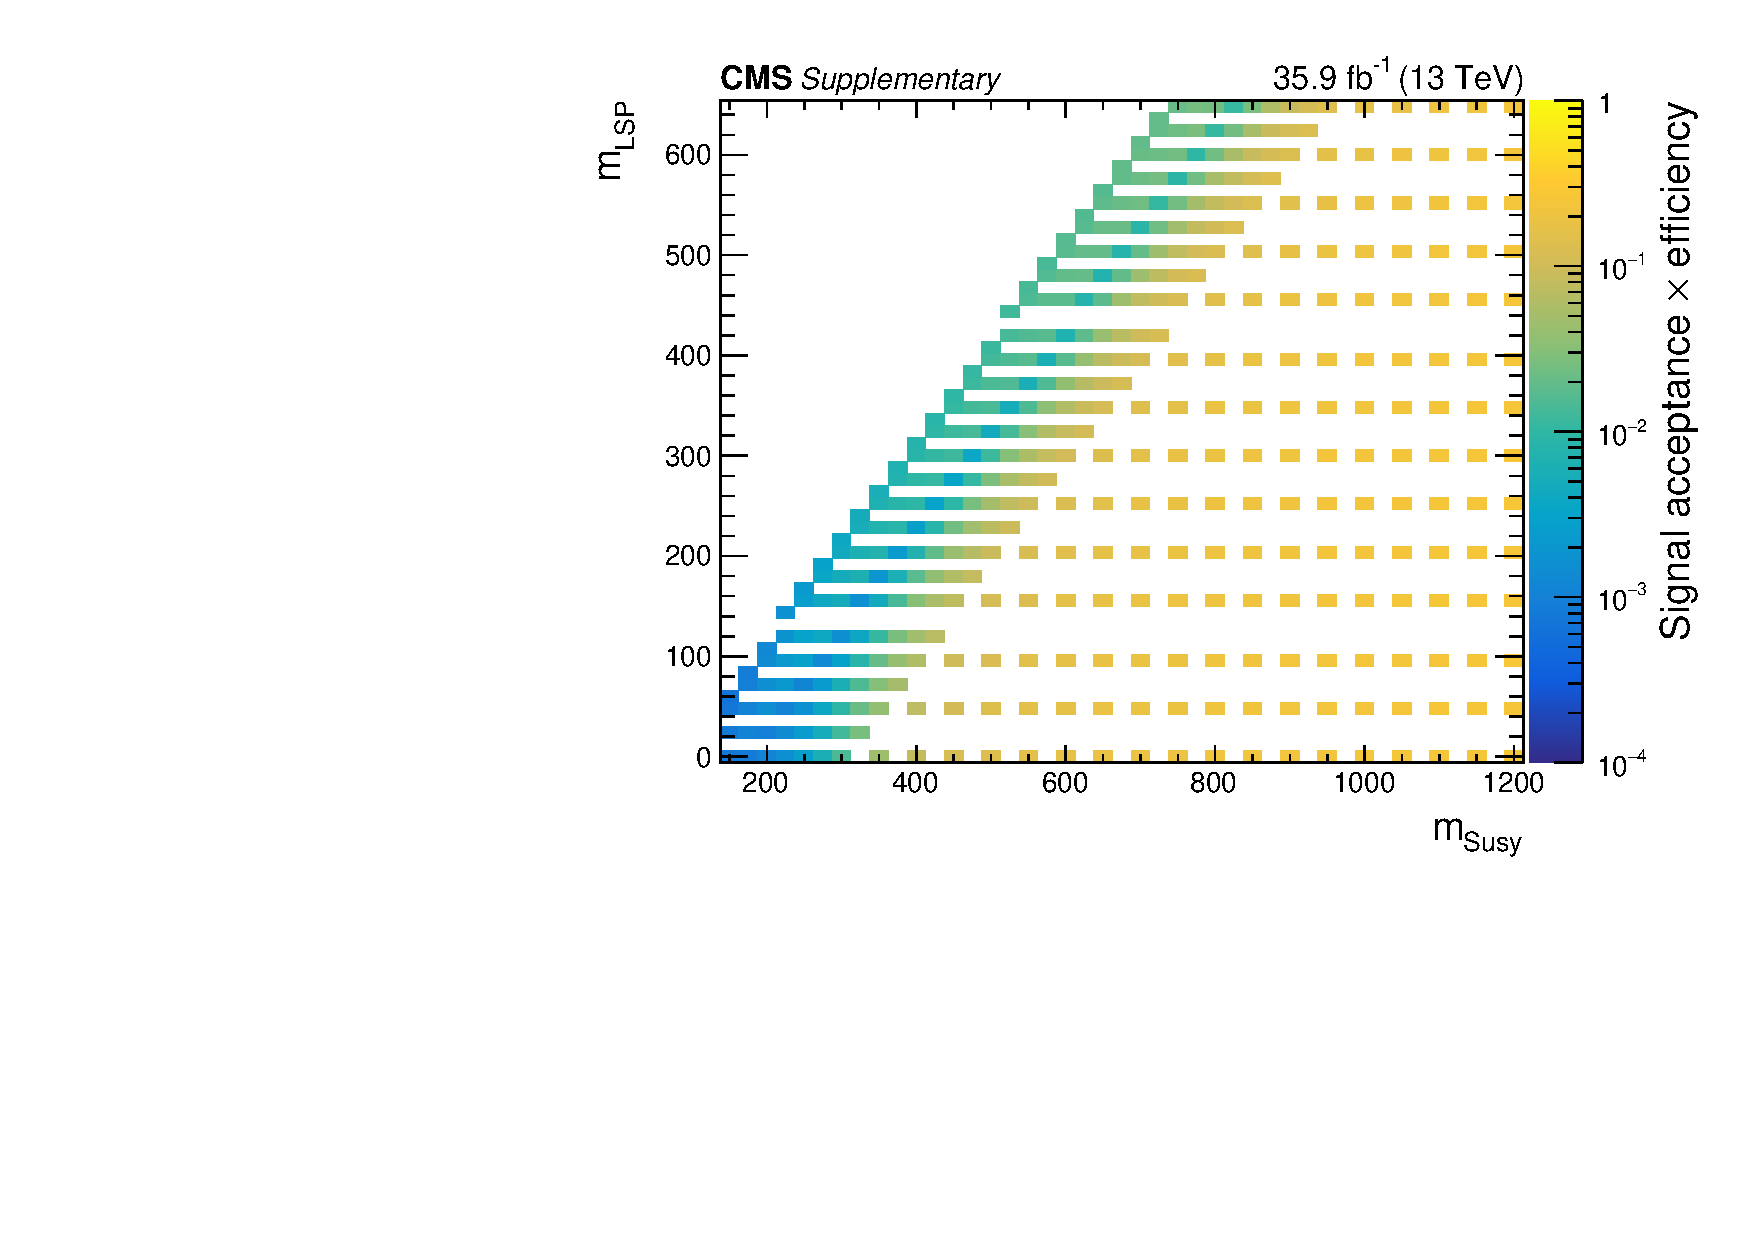
\includegraphics[width=0.52\textwidth]{Supplementary/T2ttEFF_aux}
            \label{fig:T2tt_eff}
        }
        \caption{The 95\% C.L. observed upper limit on the cross section
            (heat-map), with the expected (solid black line) observed
            (solid red line) exclusion contours, and the signal acceptance
            including all jet categories for the T2tt model.
        }
        \label{fig:T2tt}
    \end{center}
\end{figure}

\begin{figure}
    \begin{center}
        \subfigure[T2cc: the 95\% C.L. observed upper limit on the cross section
            (histogram), with the expected (solid black line) observed
            (solid red line) exclusion contours.]{
            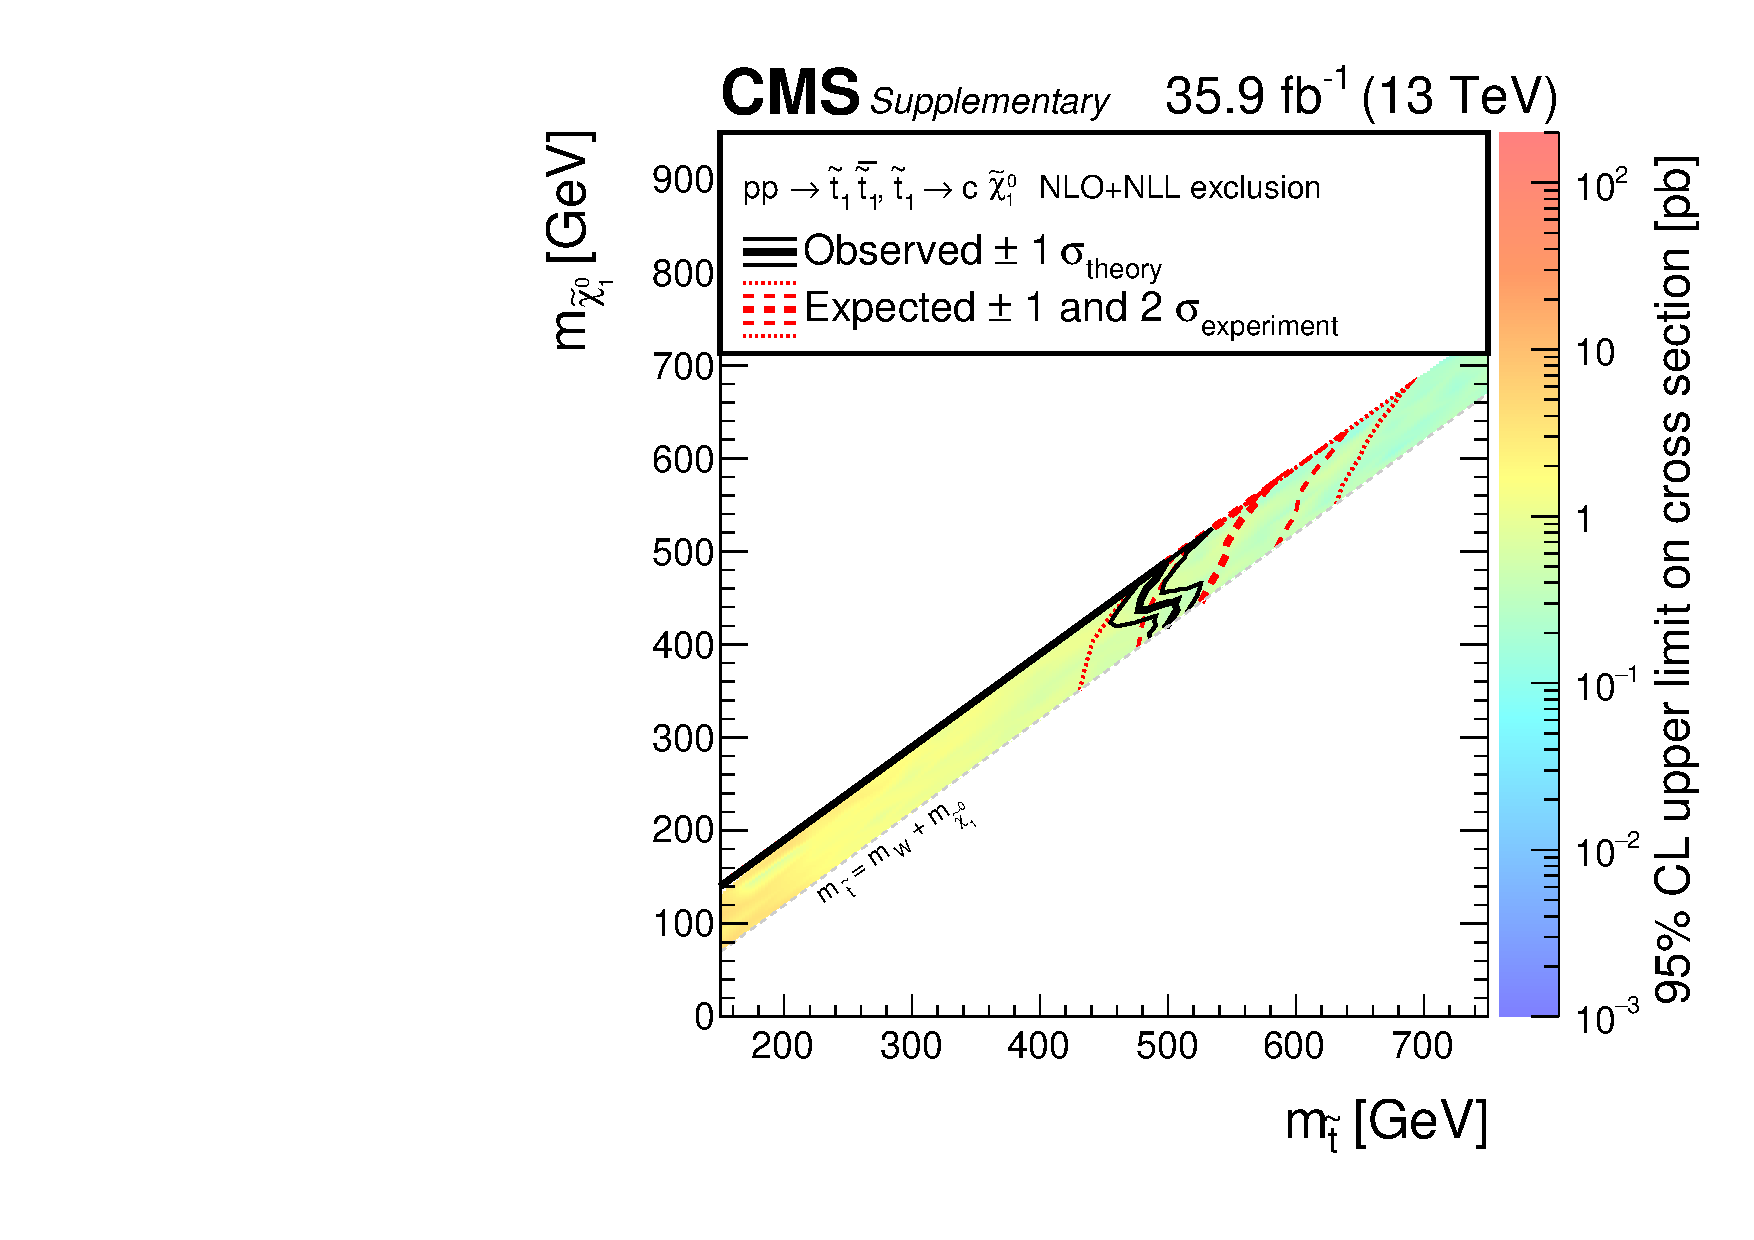
\includegraphics[width=0.4\textwidth]{Supplementary/T2ccXSEC}
            \label{fig:T2cc_excl}
        } ~~
        \subfigure[T2cc: signal acceptance
            including all jet categories.]{
            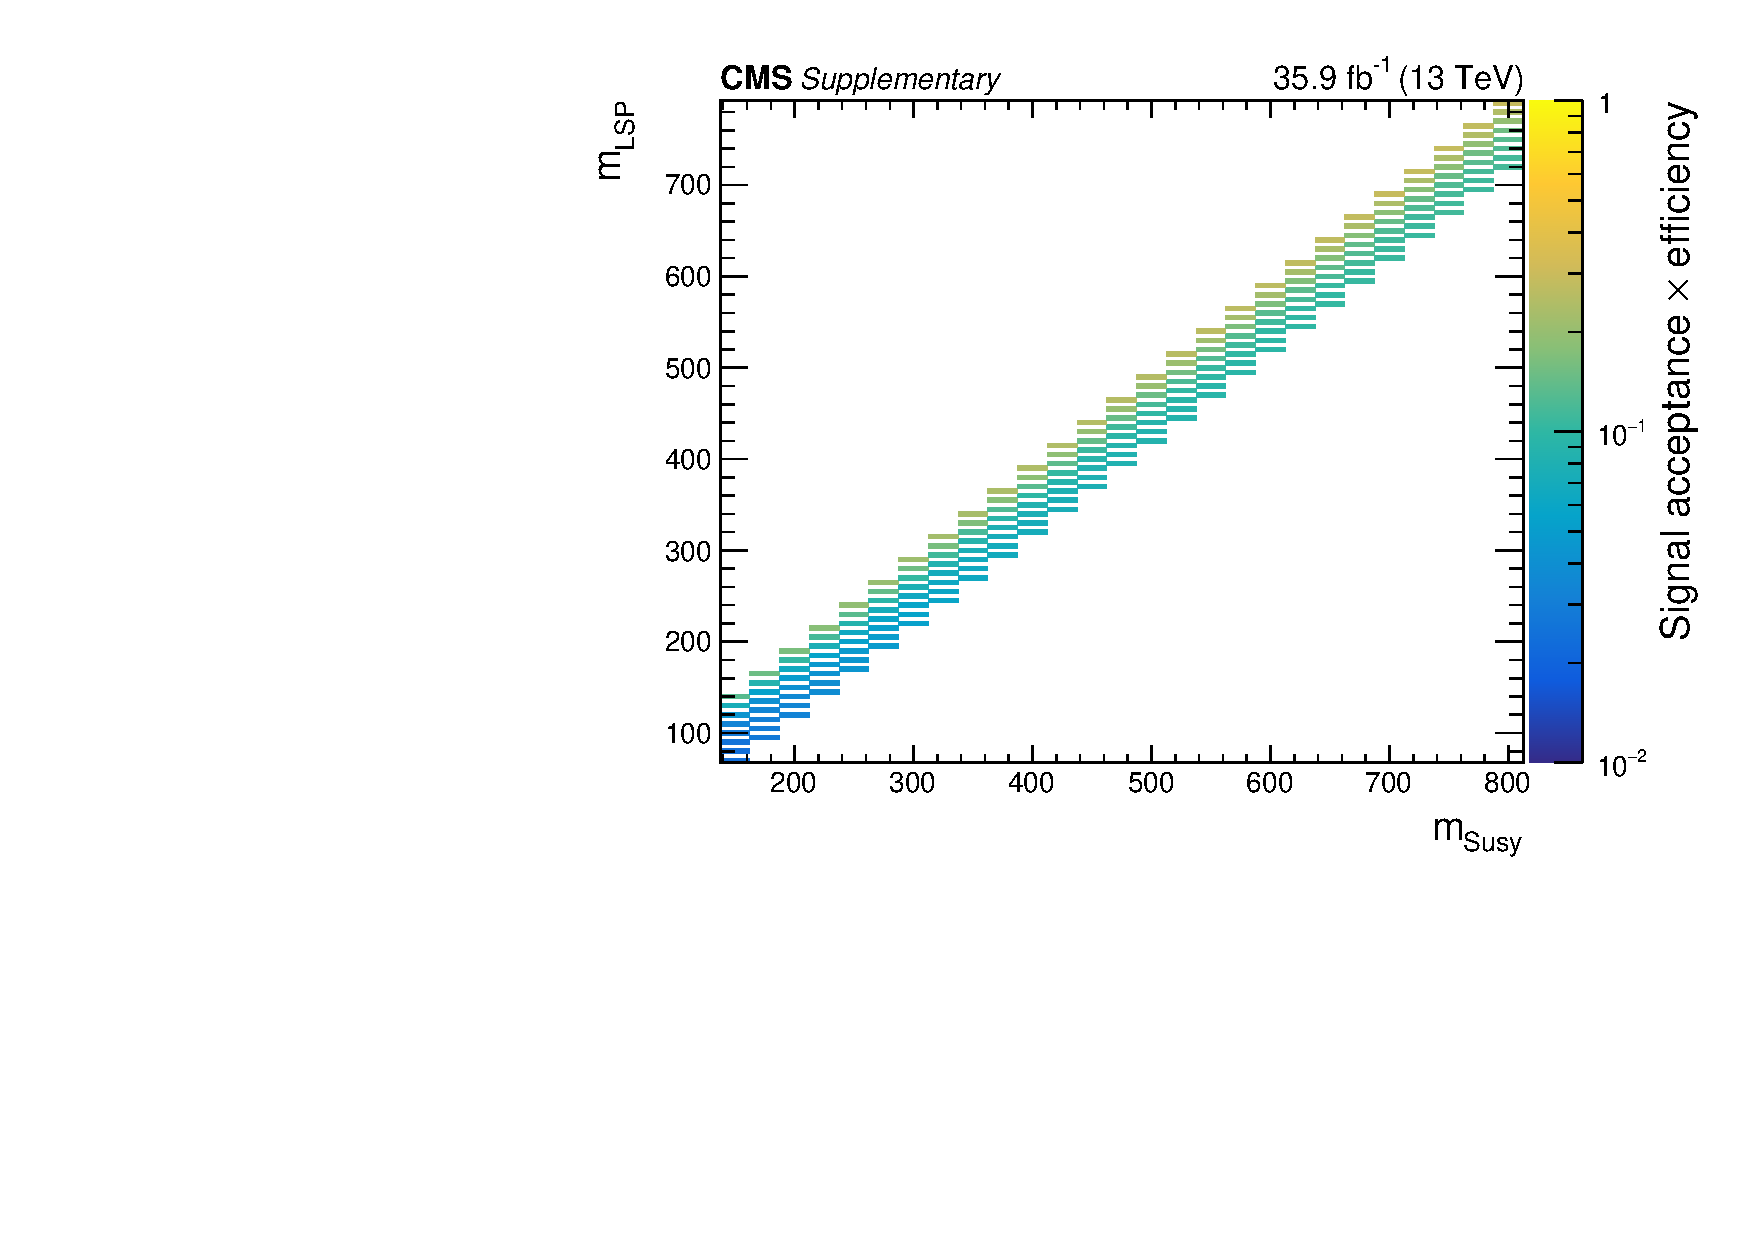
\includegraphics[width=0.52\textwidth]{Supplementary/T2ccEFF_aux}
            \label{fig:T2cc_eff}
        }
        \caption{The 95\% C.L. observed upper limit on the cross section
            (heat-map), with the expected (solid black line) observed
            (solid red line) exclusion contours, and the signal acceptance
            including all jet categories for the T2cc model.
        }
        \label{fig:T2cc}
    \end{center}
\end{figure}

\begin{figure}
    \begin{center}
        \subfigure[T2qq: the 95\% C.L. observed upper limit on the cross section
            (histogram), with the expected (solid black line) observed
            (solid red line) exclusion contours.]{
            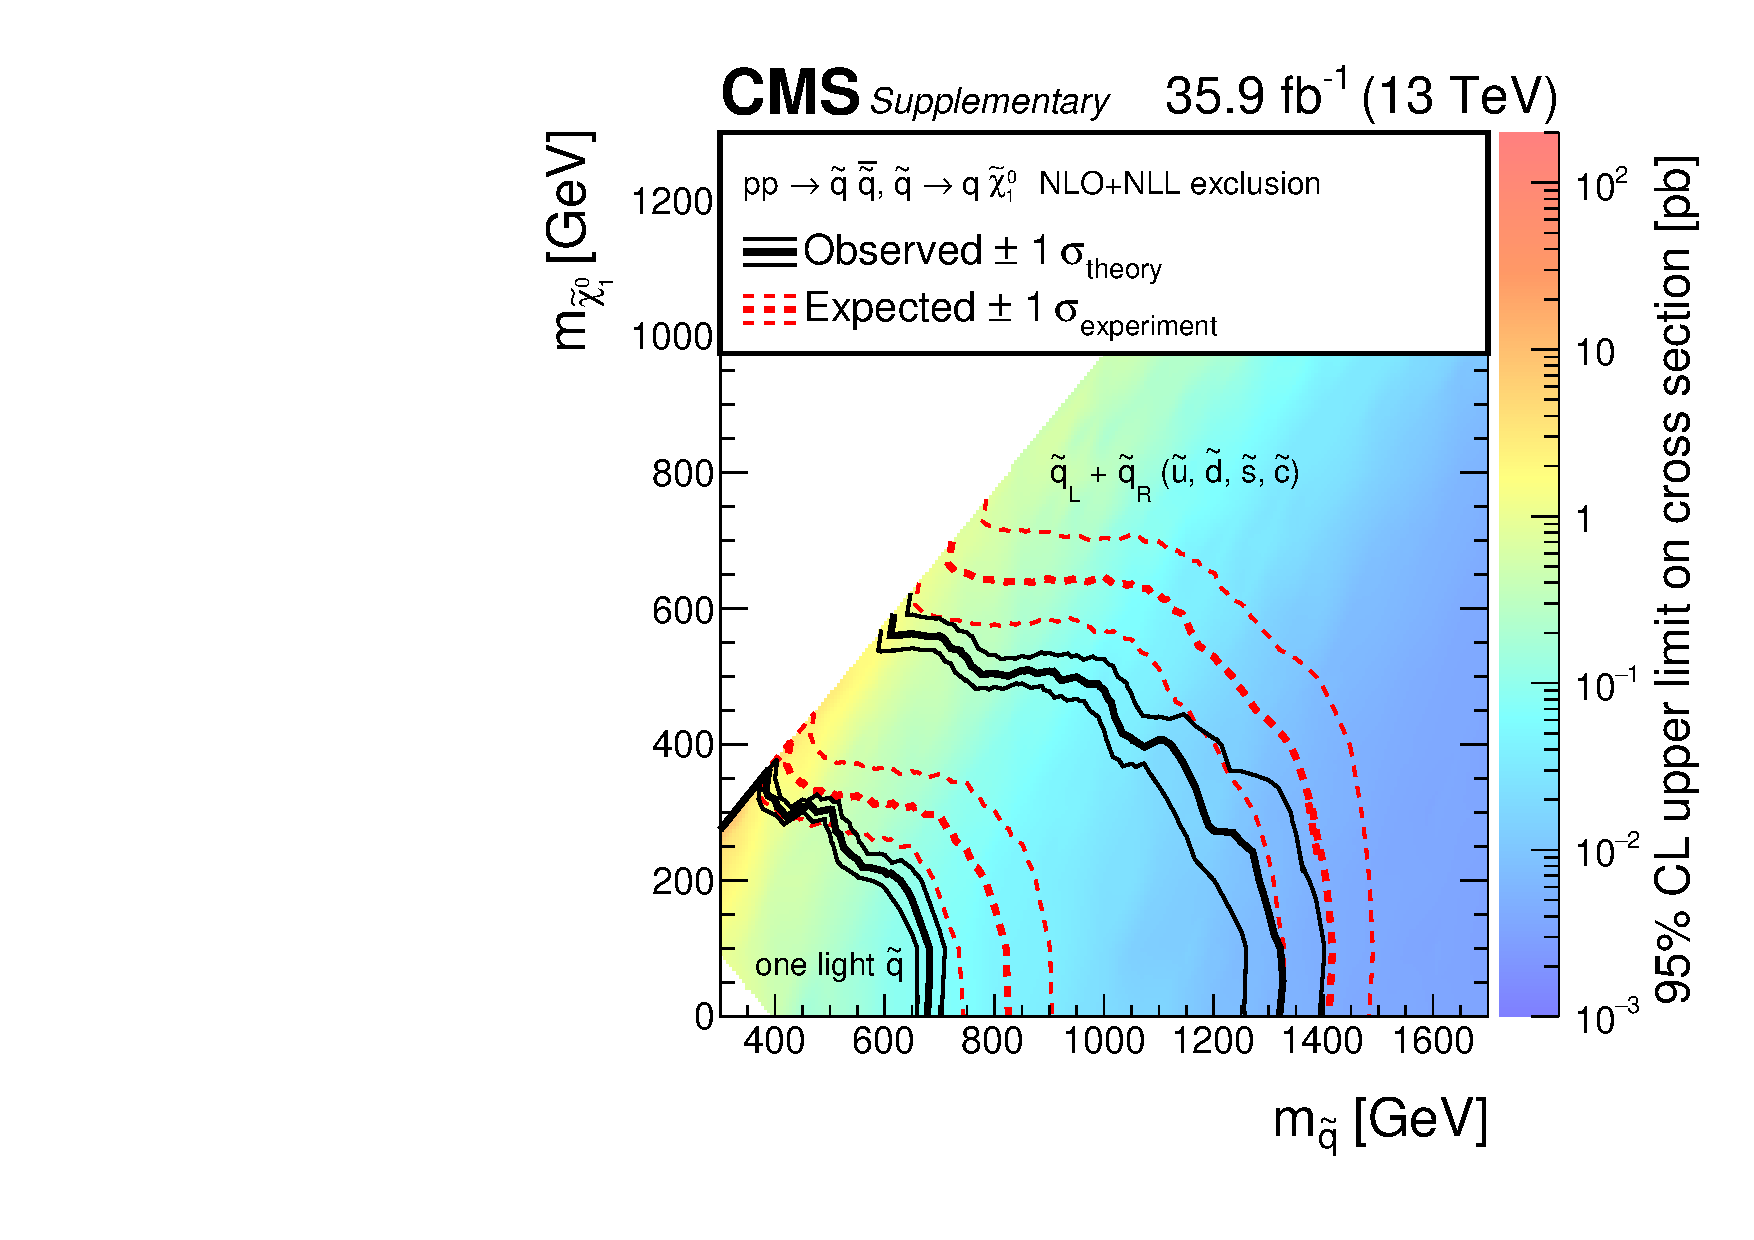
\includegraphics[width=0.4\textwidth]{Supplementary/T2qqXSEC}
            \label{fig:T2qq_excl}
        } ~~
        \subfigure[T2qq: signal acceptance
            including all jet categories.]{
            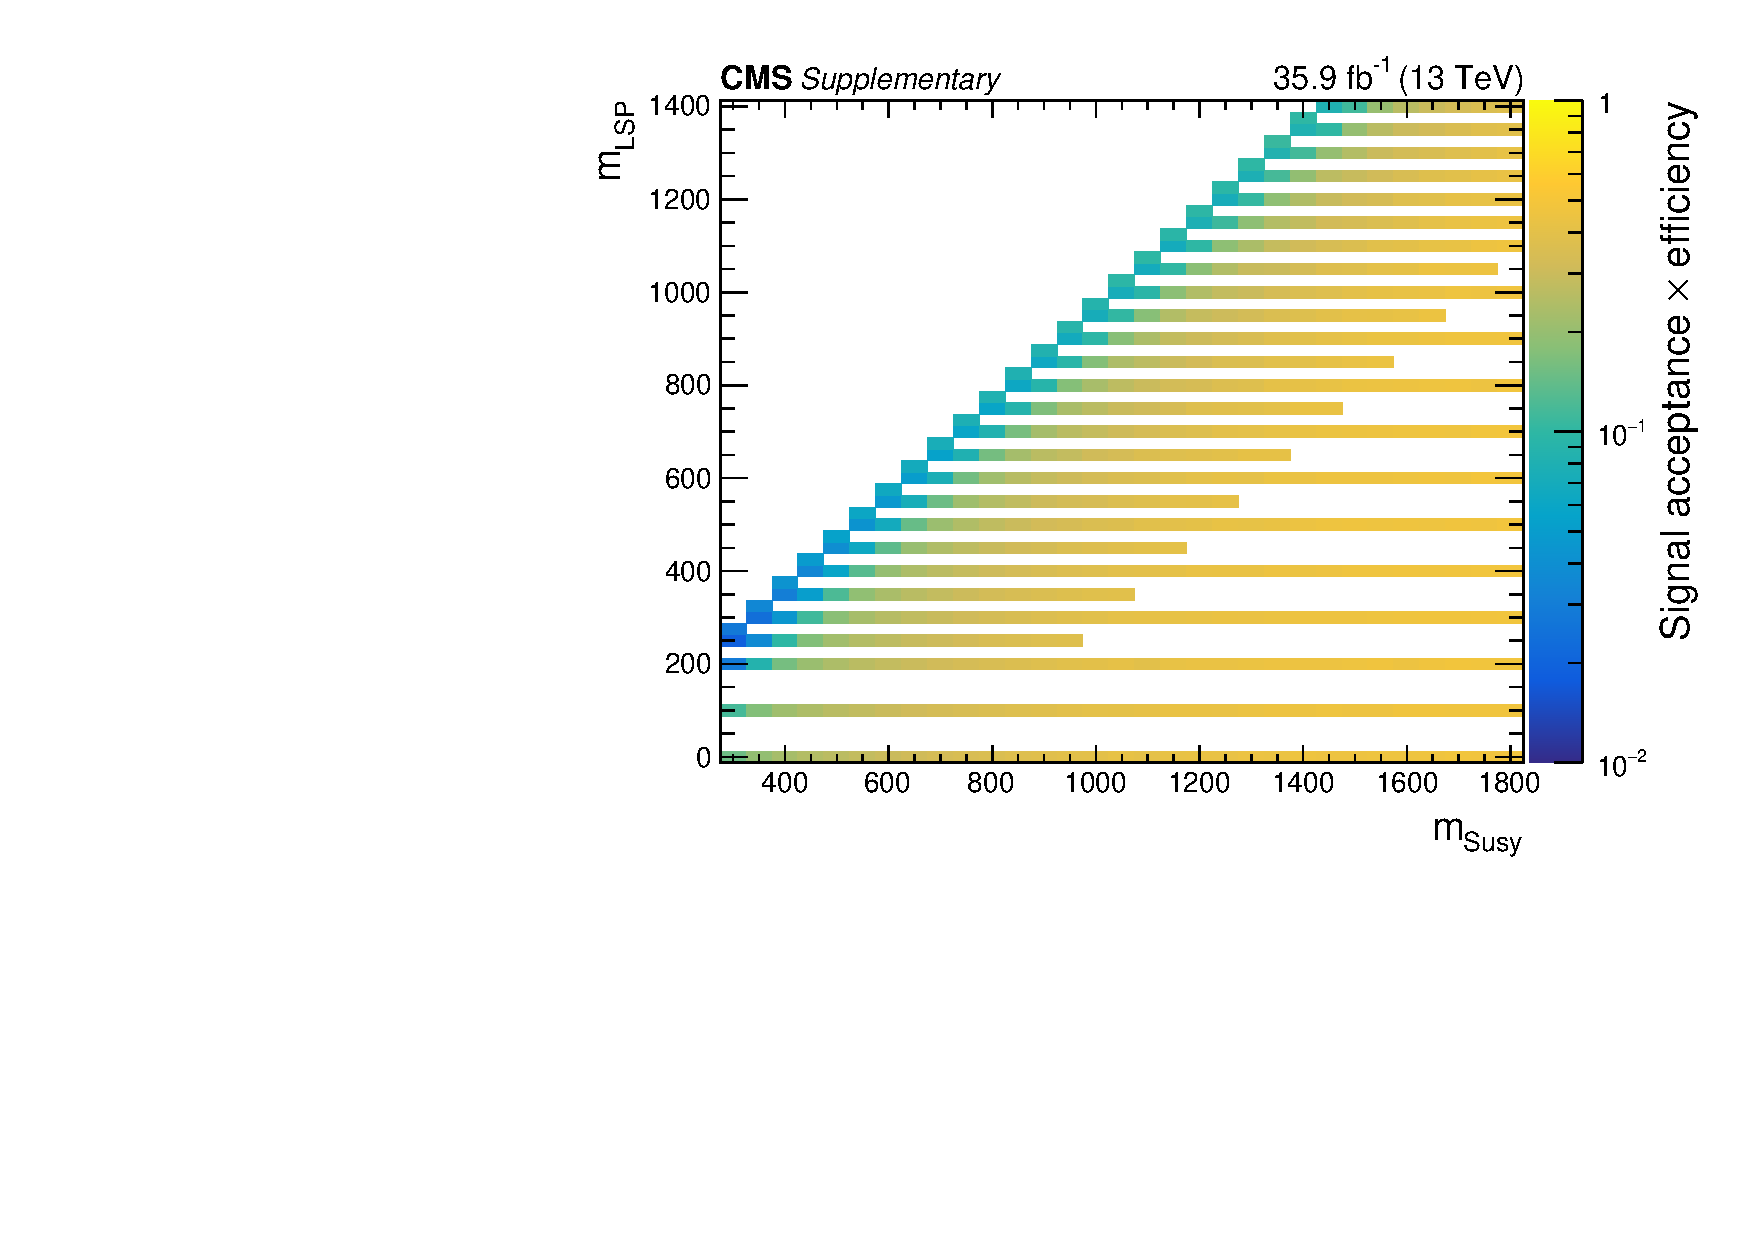
\includegraphics[width=0.52\textwidth]{Supplementary/T2qqEFF_aux}
            \label{fig:T2qq_eff}
        }
        \caption{The 95\% C.L. observed upper limit on the cross section
            (heat-map), with the expected (solid black line) observed
            (solid red line) exclusion contours, and the signal acceptance
            including all jet categories for the T2qq model.
        }
        \label{fig:T2qq}
    \end{center}
\end{figure}

\clearpage
\begin{figure}
    \begin{center}
	    \subfigure[T1qqqq (Meta-stable Gluino): the 95\% C.L. observed upper limit on the cross section
            (histogram), with the expected (solid black line) observed
            (solid red line) exclusion contours.]{
            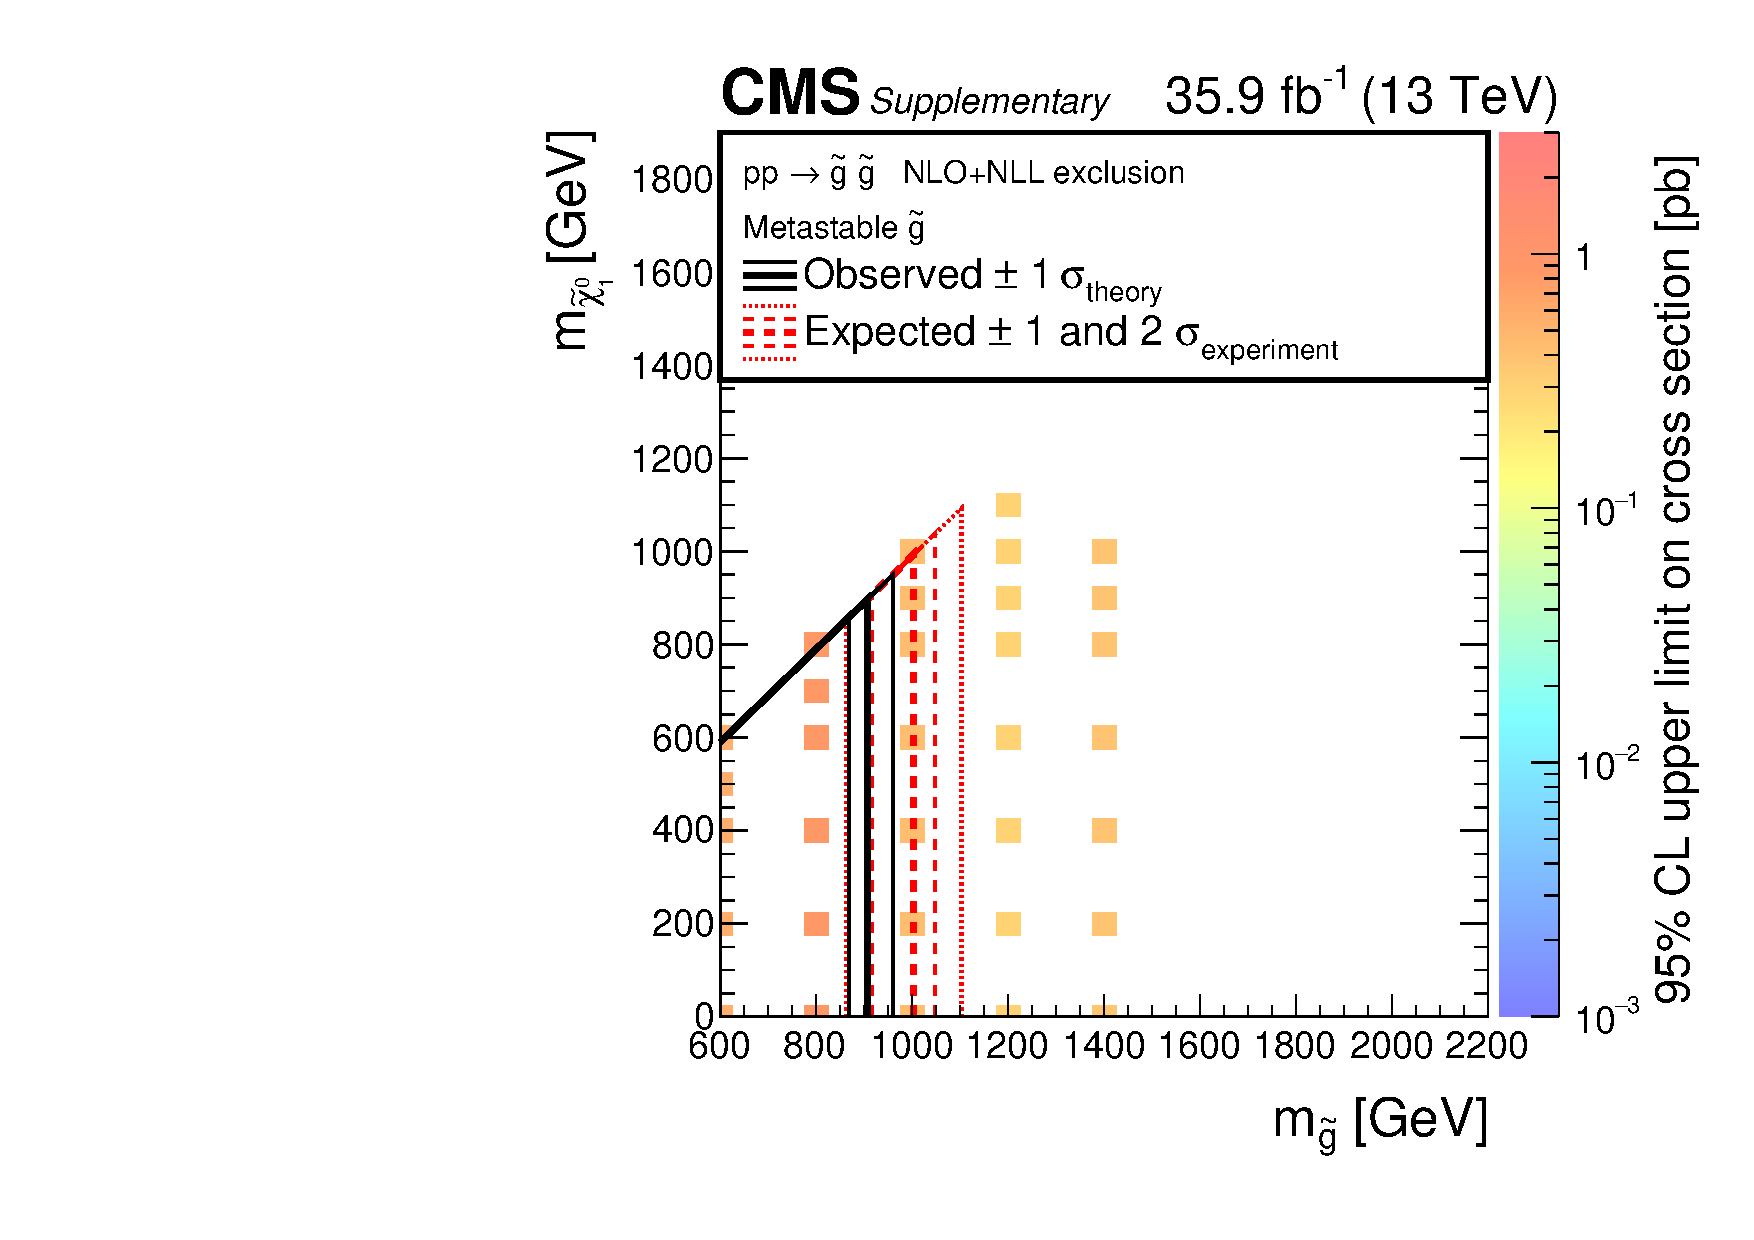
\includegraphics[width=0.4\textwidth]{Supplementary/T1qqqqLLStableXSEC}
            \label{fig:T1qqqqLL_excl}
        } ~~
	    \subfigure[T1qqqq (Meta-stable Gluino): signal acceptance
            including all jet categories.]{
	    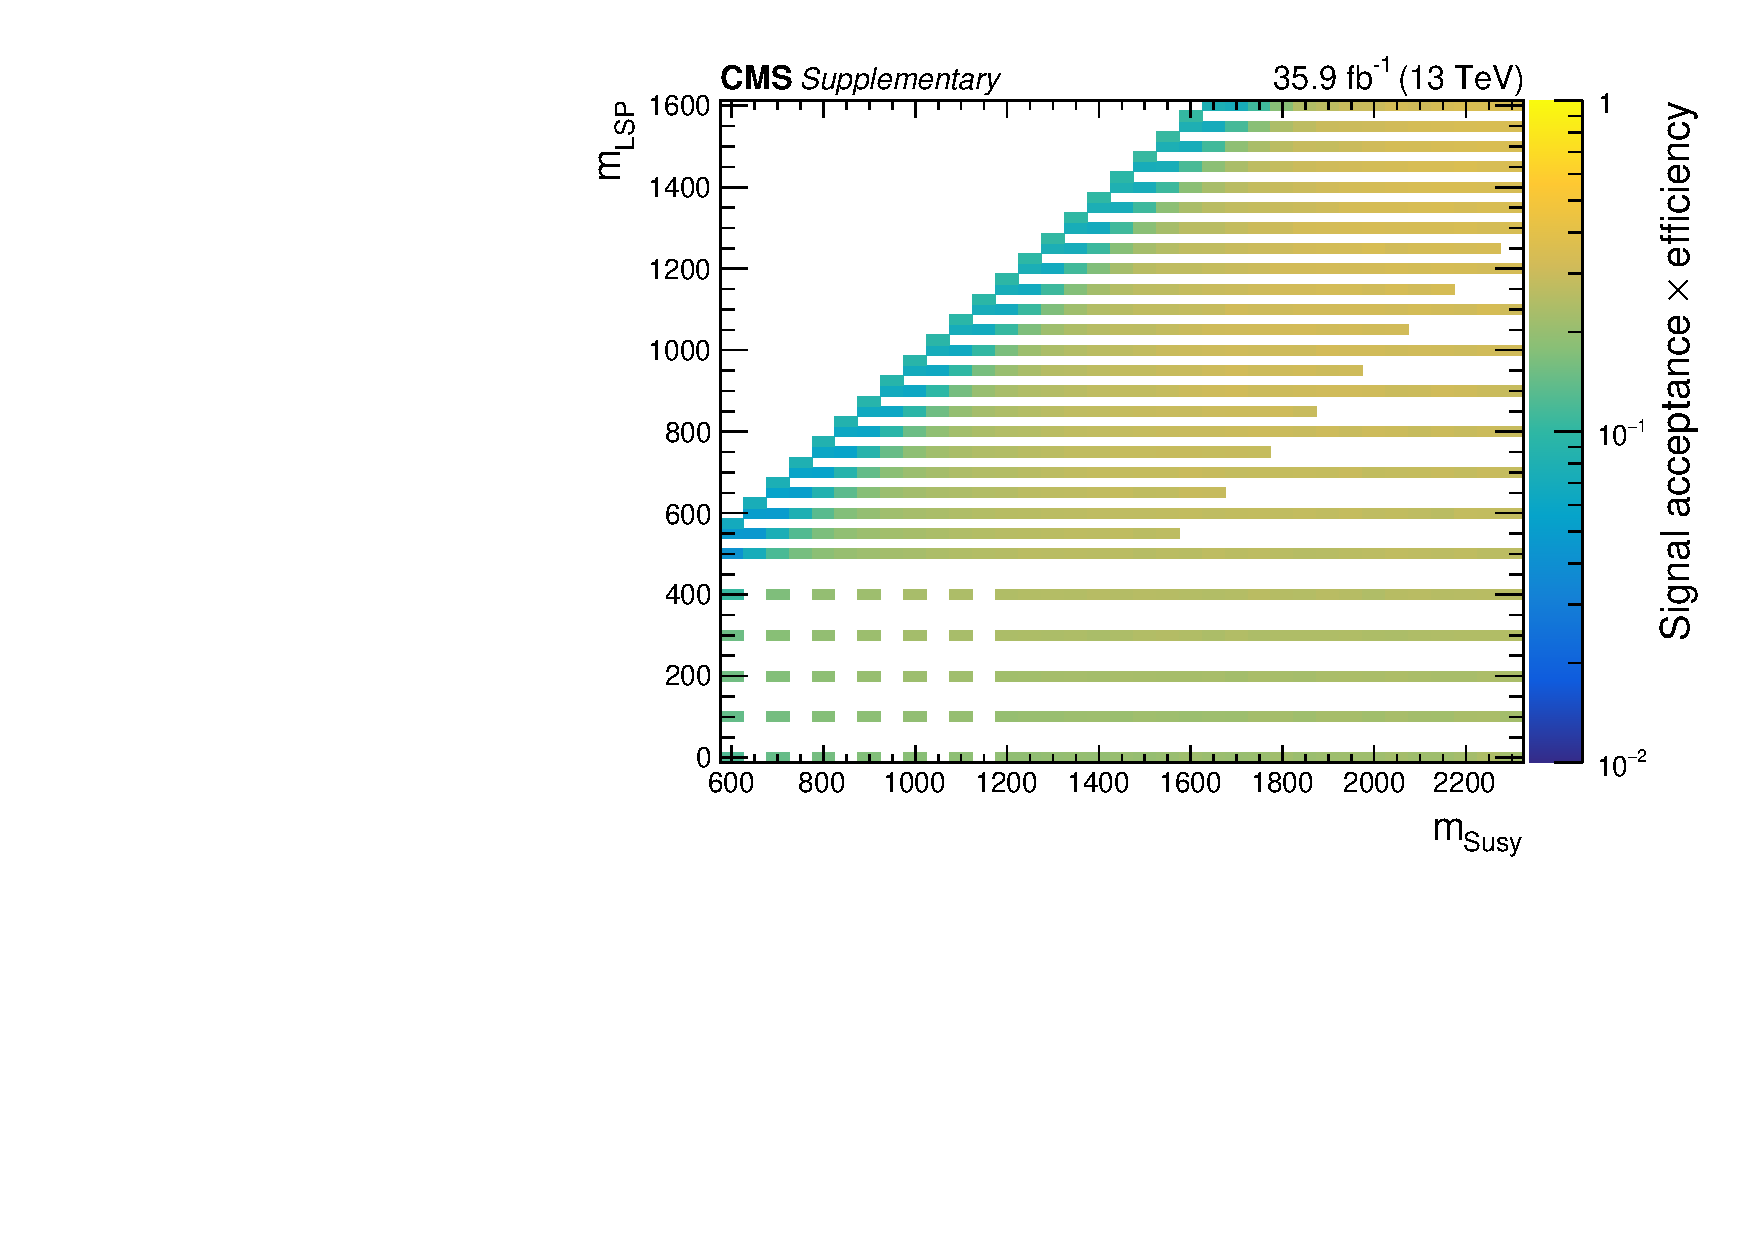
\includegraphics[width=0.52\textwidth, draft]{Supplementary/T1qqqqEFF_aux}
            \label{fig:T1qqqqLL_eff}
        }
        \caption{The 95\% C.L. observed upper limit on the cross section
            (heat-map), with the expected (solid black line) observed
            (solid red line) exclusion contours, and the signal acceptance
	    including all jet categories for the T1qqqq (with meta-stable gluinos) model.
        }
        \label{fig:T1qqqqLL}
    \end{center}
\end{figure}

\clearpage
\begin{figure}[!t]
  \centering
  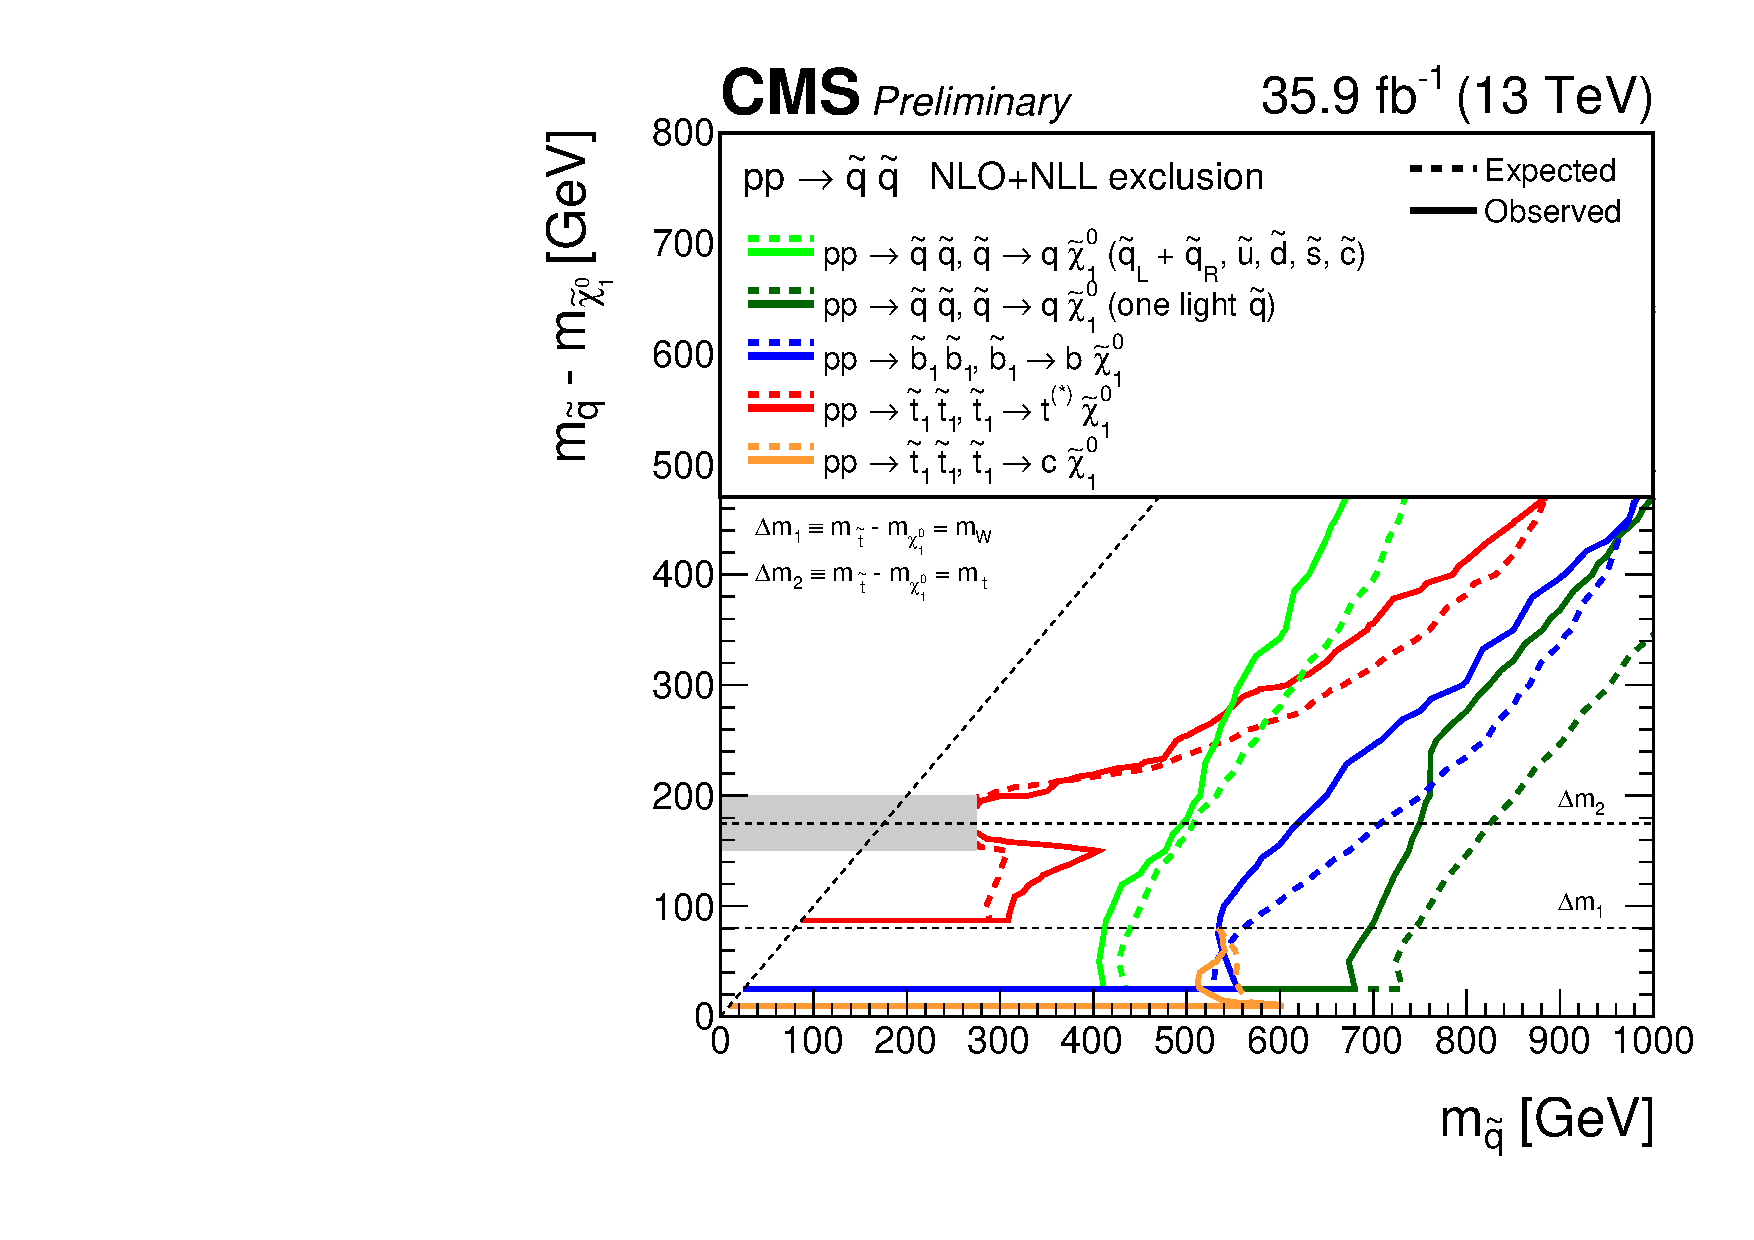
\includegraphics[width=0.6\textwidth]{Supplementary/squarkZoomSUMMARY_transpose}\\
  \caption{Observed and expected mass exclusions at 95\% CL
    (indicated, respectively, by solid and dashed contours) for
    simplified models with an intermediate squark.
    Five model families involve the direct pair
    production of squarks. The first scenario considers the pair
    production and decay of bottom squarks (\texttt{T2bb}). Two
    scenarios involve the production and decay of top squark pairs
    (\texttt{T2tt} and \texttt{T2cc}). The grey shaded region denotes
    \texttt{T2tt} models that are not considered for
    interpretation. Two further scenarios involve, respectively, the 
    production and decay of light-flavour squarks, with different
    assumptions on the mass degeneracy of the squarks as described in
    the text (\texttt{T2qq\_8fold} and \texttt{T2qq\_1fold}).}
  \label{fig:limits-sms_aux_squarks} 
\end{figure}

\begin{figure}[!t]
  \centering
  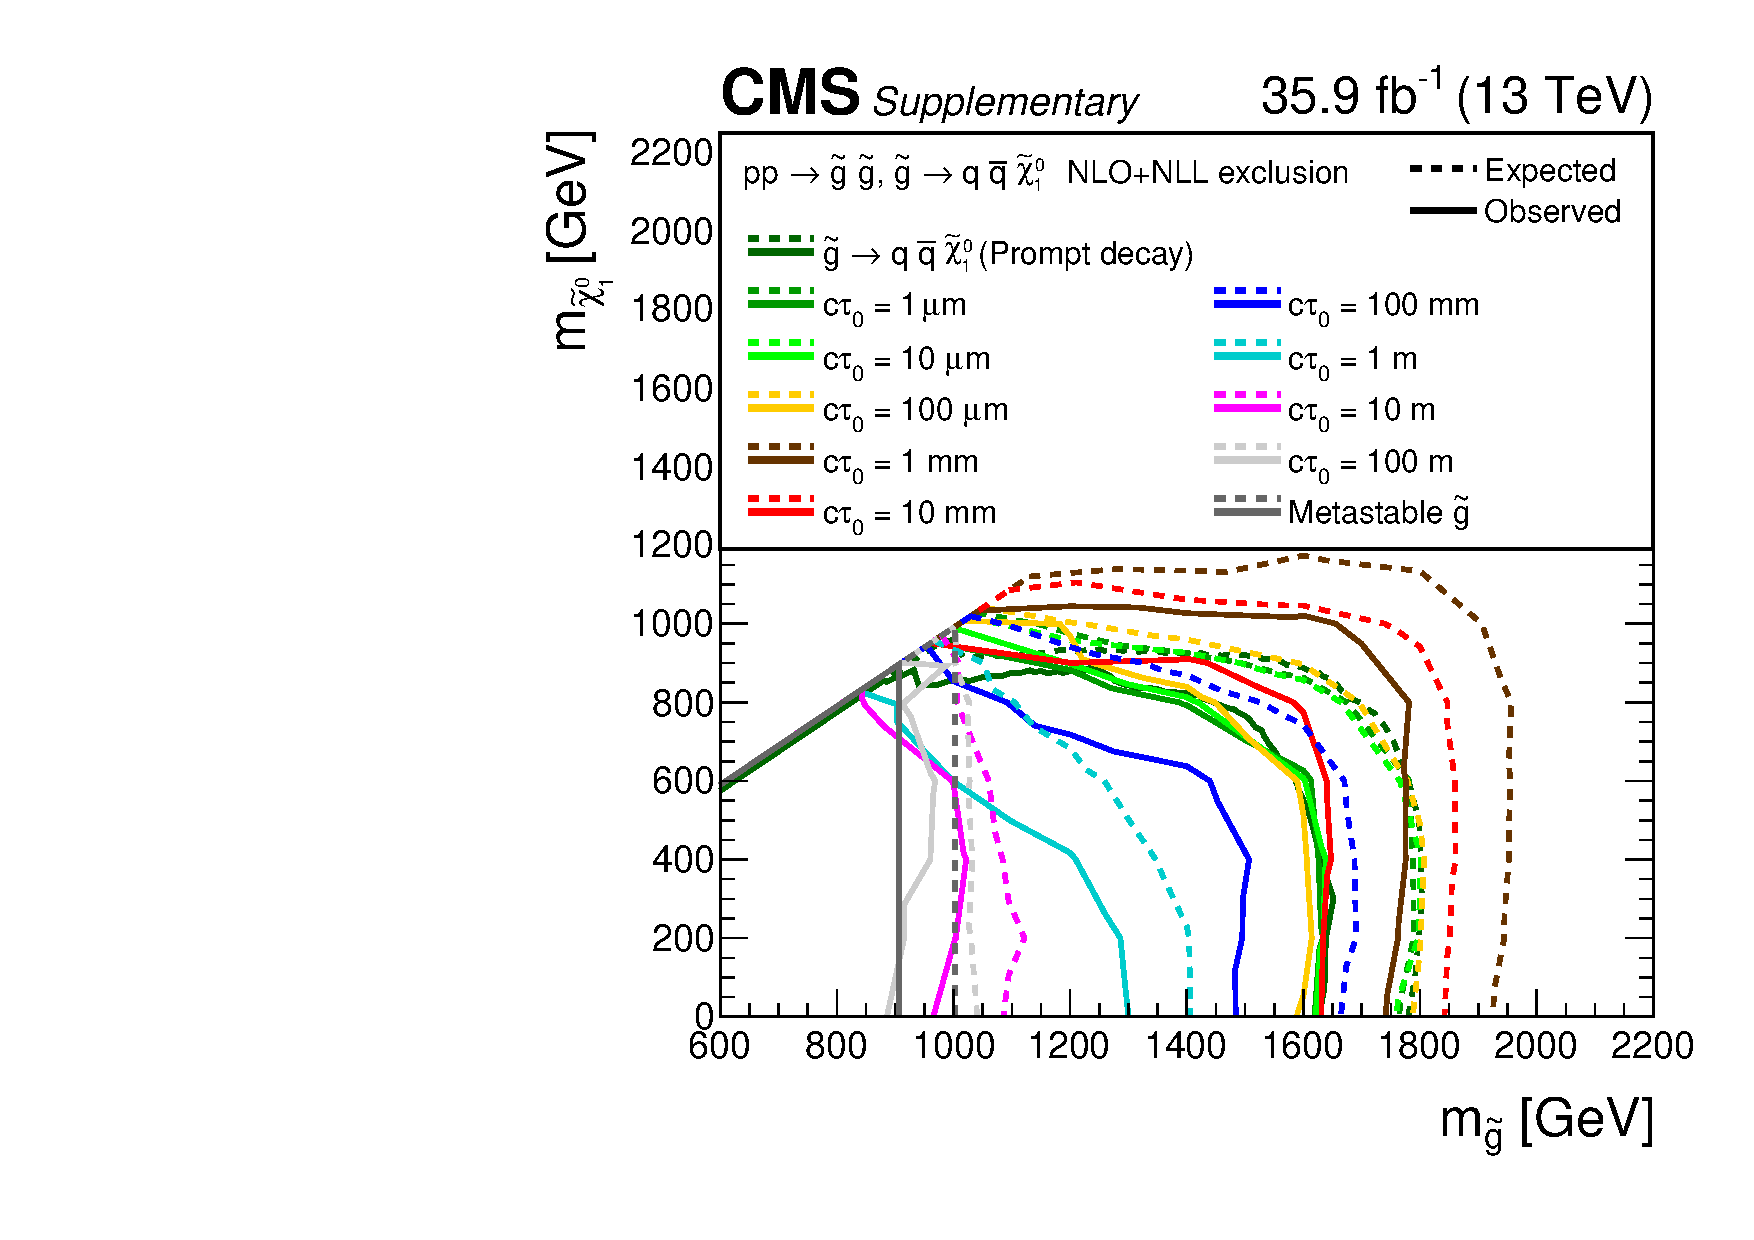
\includegraphics[width=0.6\textwidth]{Supplementary/splitAllSUMMARY}\\
  \caption{Observed and expected mass exclusions at 95\% CL
    (indicated, respectively, by solid and dashed contours) for
    the split-SUSY simplified models with all considered values of the gluino lifetime.}
  \label{fig:limits-sms_aux_long_lived} 
\end{figure}

